\documentclass[letterpaper]{article} % DO NOT CHANGE THIS
\usepackage[submission]{aaai2027}  % DO NOT CHANGE THIS
\usepackage[hyphens]{url}  % DO NOT CHANGE THIS
\usepackage{graphicx} % DO NOT CHANGE THIS
\urlstyle{rm} % DO NOT CHANGE THIS
\def\UrlFont{\rm}  % DO NOT CHANGE THIS
\usepackage{natbib}  % DO NOT CHANGE THIS AND DO NOT ADD ANY OPTIONS TO IT
\usepackage{caption} % DO NOT CHANGE THIS AND DO NOT ADD ANY OPTIONS TO IT
\frenchspacing  % DO NOT CHANGE THIS

\usepackage{amsmath}
\usepackage{amssymb}
\usepackage{algorithm}
\usepackage{algpseudocode}
\usepackage{subcaption}
\usepackage{tabularx}
\usepackage{listings}
\usepackage{multirow}
\usepackage{booktabs}

\pdfinfo{
/TemplateVersion (2027.1)
}

\setcounter{secnumdepth}{0}

\title{FlowKG: Generative Knowledge Graph Refinement via Flow Matching for Recommendation}
\author{Anonymous Submission}
\affiliations{}

\begin{document}

\maketitle

\begin{abstract}
	Incorporating Knowledge Graphs (KGs) into recommender systems has become a de facto standard for alleviating data sparsity and the cold-start problem. While Graph Neural Networks have shown success in this domain, current approaches face two critical bottlenecks. First, prevalent cascaded architectures tightly couple the KG and user-item graphs, inevitably amplifying inherent structural noise (e.g., high-entropy ``one-to-many'' relations) and propagating it into user preference modeling. Second, while generative recommendation has gained traction, existing diffusion-based methods rely on Stochastic Differential Equations (SDEs) to generate discrete graph structures. This process is not only computationally demanding but also indirect, as the ultimate goal is to refine latent representations rather than graph topology. To address these challenges, we propose FlowKG, a novel framework that integrates Decoupled Structure Learning with Flow Matching (FM) for robust and efficient recommendation. We introduce an Entropy-Guided Structure Learning module that combines structural entropy priors with learnable semantic posteriors to adaptively assess triplet quality before aggregation, ensuring high-fidelity input for a Decoupled Dual-View Encoder. Furthermore, we shift the generative paradigm from SDE-based diffusion to FM. By constructing deterministic Ordinary Differential Equation trajectories based on Optimal Transport, FlowKG evolves noisy item embeddings directly towards the target semantic manifold along straight, stable paths. We conduct extensive experiments on four publicly available datasets, consistently demonstrating the superiority of our FlowKG compared to various competitive baselines. Our code is available at \url{https://anonymous.4open.science/r/FlowKG}.
\end{abstract}

\section{Introduction}
\label{sec:introduction}

 % !TEX spellcheck = en_US
% !TeX root = main.tex

\begin{figure}[t]
	\centering
	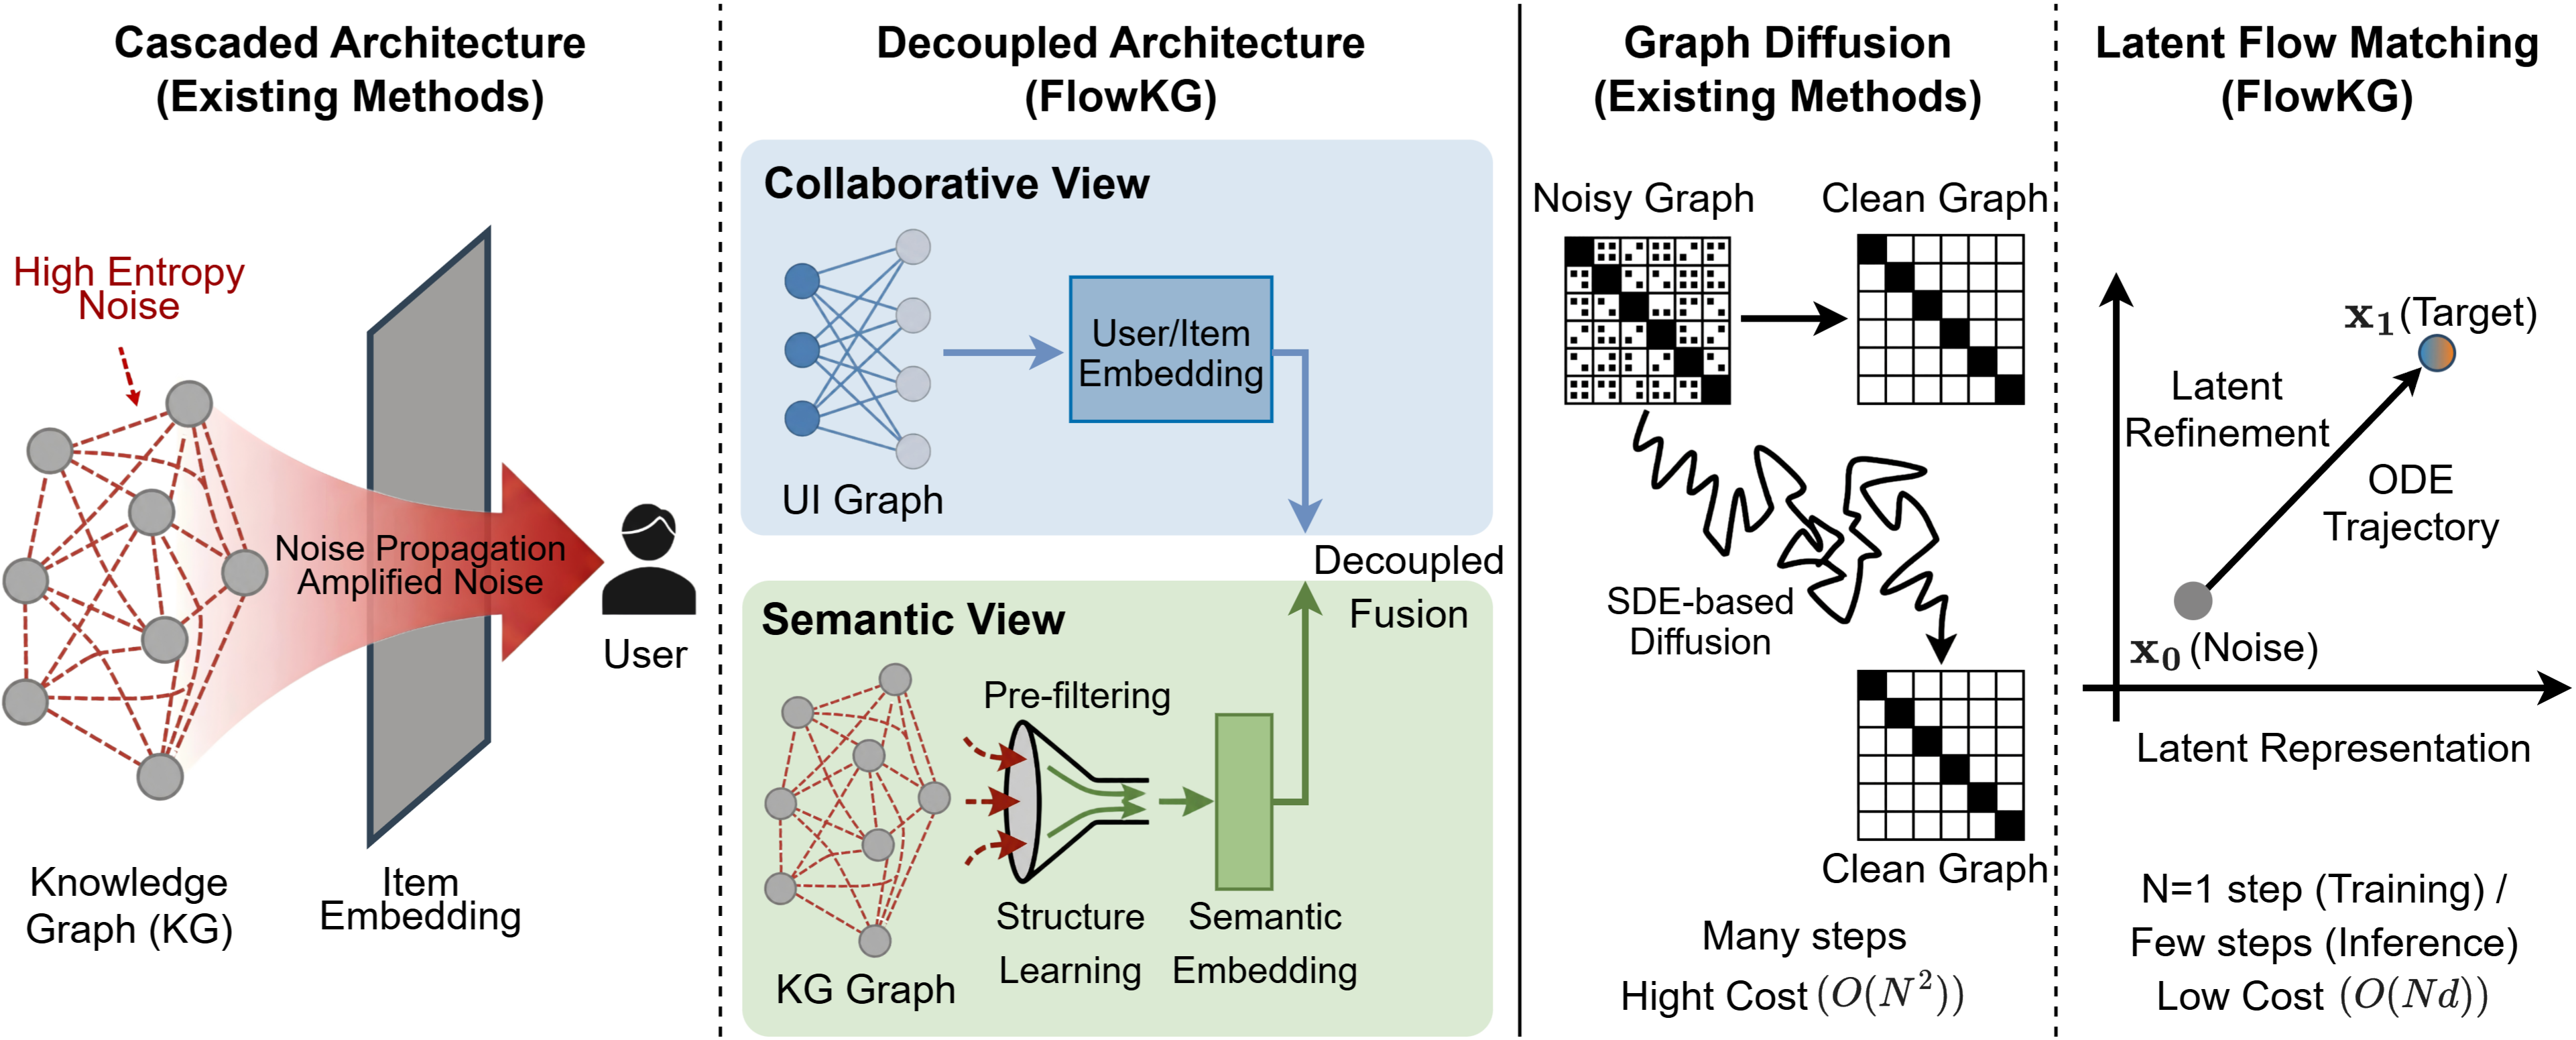
\includegraphics[width=\columnwidth]{image/motivation.png}
	\caption{\textbf{Motivation for FlowKG.} Left: Noise propagation issues. Right: The shift to ODE-based refinement.}
	\label{fig:motivation_main}
\end{figure}


In the era of information explosion, personalized recommender systems serve as pivotal tools for mitigating information overload~\cite{adomavicius2005toward,ricci2010introduction}. To mitigate long-standing challenges such as data sparsity and the cold-start problem, incorporating knowledge graphs (KGs) as auxiliary information has become a common practice~\cite{guo2020survey,zhang2016collaborative}. By mapping items to entities within a structured graph, KGs provide rich semantic connectivity (e.g., Movie-Director, Product-Brand), enabling models to reason about user preferences through high-order relations~\cite{wang2019kgat,wang2018ripplenet}.

Building upon this, Graph Neural Networks (GNNs)~\cite{wang2019kgat, wang2021learning}, renowned for their powerful ability to model graph structures, have achieved notable success in recommendation tasks. However, most existing methods adopt a  ``Cascaded Architecture'': item representations are first enriched by aggregating information from the KG and are then propagated through the user-item interaction graph for collaborative filtering. This tightly-coupled design harbors a critical flaw---noise propagation. Real-world KGs often contain numerous ``one-to-many'' high-entropy connections. For instance,  a single movie might be associated with dozens of generic tags (e.g., classic, emotional). Within a cascaded architecture, as illustrated in Figure~\ref{fig:motivation_main} (Left), such structural noise  is amplified through representation propagation, ultimately contaminating the modeling of user preferences and leading to degraded performance.

To sever this noise propagation pathway, we first propose a fundamental architectural shift: a Decoupled Dual-View Encoder. Unlike cascaded models that subordinate the collaborative signal to the semantic signal, our method processes the Collaborative View (user-item interaction graph) and the Semantic View (KG) in parallel. This design structurally insulates the collaborative learning process from direct structural interference by graph noise, allowing the model to extract clean user behavioral patterns.

Nevertheless, architectural decoupling represents only a partial solution. While it effectively severs the noise propagation path, it does not inherently address the persistent challenge of data sparsity. To combat this, modern recommenders rely on Contrastive Learning (CL)~\cite{yang2022knowledge, zou2022improving} to maximize the mutual information between views. Yet, the efficacy of CL is strictly bound by the quality of the underlying views. If the semantic view remains noisy, standard stochastic augmentations (e.g., random edge dropout) merely yield ``noisy augmented views,'' potentially enforcing the alignment of erroneous semantics. To remedy this, we introduce an Entropy-Guided Structure Learning (ESL) module at the upstream stage. By leveraging relational entropy as a structural prior, ESL identifies and prunes high-uncertainty connections before encoding and augmentation. This ensures that the self-supervised signals in CL are derived from a purified, high-fidelity structure.

Furthermore, even with a purified structure, GNN-based encoders face the inherent limitation of over-smoothing~\cite{li2018deeper,oonograph}, often yielding item representations with limited discriminative power. While recent Generative Recommendation methods (e.g., Diffusion Models~\cite{jiang2024diffkg, li2025mask}) attempt to reconstruct better distributions, they predominantly operate via ``Graph-Level Diffusion'' using Stochastic Differential Equations (SDEs). This paradigm is computationally demanding and indirect, as it generates discrete graph structures rather than optimizing the embeddings themselves. To address this, we introduce a Flow Matching Refinement module at the downstream stage. As shown in Figure~\ref{fig:motivation_main} (Right), we shift from graph diffusion to Latent Representation Refinement. By constructing deterministic Ordinary Differential Equation (ODE) paths based on Optimal Transport, we directly and efficiently rectify item embeddings, evolving them from a noisy distribution to a robust target semantic manifold.

In summary, we propose FlowKG, a holistic framework that integrates decoupled architecture, upstream structure purification, and downstream representation refinement. The main contributions of this work can be summarized  as follows:

\begin{itemize}
	\item \textbf{Novel Architecture:} We identify the noise propagation issue in cascaded architectures and propose a Decoupled Dual-View Encoder to process semantic and collaborative signals in parallel, effectively preventing mutual interference.
	\item \textbf{Methodological Innovation:} We propose a two-stage denoising paradigm: (1) Upstream Entropy-Guided Structure Learning (ESL) to purify the graph structure before contrastive augmentation, and (2) Downstream Flow Matching Refinement to efficiently rectify latent item representations via deterministic ODE paths.
	\item \textbf{SOTA Performance:} Extensive experiments on four benchmark datasets demonstrate that FlowKG significantly outperforms state-of-the-art baselines. The results validate its robustness against noise, as well as its superior training efficiency.
\end{itemize}



\section{Related work}
\label{sec:relatedwork}
\subsection{Knowledge-aware Recommendation}
Knowledge-aware recommendation has evolved significantly, aiming to alleviate data sparsity by incorporating external KGs. Early embedding-based methods~\cite{zhang2016collaborative,cao2019unifying,wang2018dkn} primarily utilized TransR or auto-encoders to extract semantic features from KGs to enrich item representations.
Subsequently, propagation-based methods~\cite{wang2019kgat,wang2021learning,yang2022knowledge,yang2023knowledge,zou2022improving,zou2024knowledge,li2025hypercomplex,li2025lightkg} emerged as the dominant paradigm. For instance, KGAT~\cite{wang2019kgat} employs graph attention mechanisms to recursively propagate embeddings across high-order neighbors, explicitly modeling connectivity. KGIN~\cite{wang2021learning} further refines this by disentangling user intents behind interactions via relational paths.
To tackle the inherent noise in KGs, recent advancements have introduced CL~\cite{zou2022improving,yang2023knowledge}. KGIC~\cite{zou2022improving} and KGRec~\cite{yang2023knowledge} construct multi-view contrastive tasks or leverage rationalization scores to denoise supervision signals.
However, most existing approaches adopt a cascaded architecture where KG embeddings are aggregated before collaborative interaction modeling. This tight coupling inevitably propagates structural noise (e.g., high-entropy relations) into the user preference learning process, limiting the robustness of the final representations.

\subsection{Generative Models for Recommendation}
Generative models, particularly diffusion models, have recently garnered attention in recommender systems for their superior ability to model complex distributions~\cite{lin2025diffusion,wei2025diffusion}. Methods like DiffKG~\cite{jiang2024diffkg} and KMDCL~\cite{li2025mask} apply diffusion processes to reconstruct KGs or generate denoised views, achieving state-of-the-art performance. Despite their success, diffusion models suffer from slow inference speeds due to multi-step SDE sampling and often require computationally expensive graph-level generation.
To overcome these efficiency bottlenecks, FM~\cite{lipman2023flow} has been introduced as a more efficient Continuous Normalizing Flow paradigm based on deterministic ODEs. Recent works have successfully adapted FM to various recommendation scenarios: FlowCF~\cite{liu2025flow} applies discrete flow matching to collaborative filtering; FlowRec~\cite{li2025preference} and FMREC~\cite{ijcai2025p346} utilize FM to model dynamic user preference trajectories in sequential recommendation; RecFlow~\cite{huangflow} addresses anisotropic noise in social recommendation.
Nevertheless, the potential of Flow Matching in Knowledge-aware Recommendation remains unexplored. Existing FM-based recommenders typically focus on homogeneous graphs or user sequences, failing to address the unique challenges of KGs, such as the heterogeneity of relations and the prevalence of one-to-many structural noise.

\section{Preliminaries}
\label{sec:preliminaries}
%在本节中，我们首先对知识图谱增强的推荐问题进行形式化定义。随后，我们简要介绍流匹配（Flow Matching）理论，特别是基于最优传输路径的条件流匹配，这构成了本文生成式增强模块的数学基础。
%
%\subsection{Problem Formulation}
%我们将知识图谱推荐任务建模为异构信息网络中的链路预测与排序问题。
%
%\subsubsection{User-Item Interaction Graph}
%令 $\mathcal{U} = \{u_1, u_2, \dots, u_M\}$ 表示用户集合，$\mathcal{I} = \{i_1, i_2, \dots, i_N\}$ 表示物品集合，其中 $M$ 和 $N$ 分别为用户和物品的数量。用户与物品的历史交互数据被构建为一个二部图 $\mathcal{G}_{ui} = (\mathcal{U} \cup \mathcal{I}, \mathcal{E}_{ui})$，其中边集 $\mathcal{E}_{ui}$ 包含所有观察到的交互对 $(u, i)$（即隐式反馈 $y_{ui}=1$）。
%
%\subsubsection{Knowledge Graph (KG)}
%为了引入外部语义信息，我们利用知识图谱 $\mathcal{G}_{kg} = (\mathcal{E}, \mathcal{R}, \mathcal{T})$。其中 $\mathcal{E}$ 为实体集合，$\mathcal{R}$ 为关系集合，$\mathcal{T} = \{(h, r, t) | h, t \in \mathcal{E}, r \in \mathcal{R}\}$ 为三元组集合。在推荐场景中，物品集合通常与实体集合存在映射关系，即 $\mathcal{I} \subseteq \mathcal{E}$。KG 为物品提供了丰富的语义上下文（如“电影-导演”、“商品-品牌”等关联）。
%
%\subsubsection{Task Definition}
%给定交互图 $\mathcal{G}_{ui}$ 和知识图谱 $\mathcal{G}_{kg}$，我们的目标是学习一个评分函数 $\hat{y}_{ui} = f_\Theta(u, i)$，用于预测用户 $u$ 对未交互物品 $i$ 的偏好概率。基于该预测分数，系统将为每个用户生成一个按偏好降序排列的 Top-$K$ 推荐列表。
%
%\subsection{Flow Matching for Generative Modeling}
%流匹配（Flow Matching, FM）\cite{lipman2022flow} 是一种基于连续归一化流（CNF）的生成范式，旨在通过回归固定概率路径的向量场（Vector Field）来实现分布映射。与扩散模型相比，FM 避免了复杂的随机微分方程模拟，提供了更确定性的生成轨迹和更稳定的训练目标。
%
%\subsubsection{Continuous Normalizing Flows via ODE}
%FM 将样本生成过程建模为随时间 $t \in [0, 1]$ 变化的概率密度路径 $p_t(x)$。该过程由常微分方程（ODE）描述：
%\begin{equation}
%	\frac{\mathrm{d}x_t}{\mathrm{d}t} = v_t(x_t; \theta), \quad x_0 \sim p_0(x),
%\end{equation}
%其中 $x_t \in \mathbb{R}^d$ 是状态向量，$v_t$ 是由神经网络参数化的速度向量场，$p_0$ 是已知的先验分布（通常设为标准高斯分布 $\mathcal{N}(0, \mathbf{I})$）。通过对该 ODE 从 $t=0$ 到 $t=1$ 进行数值积分，可以将噪声 $x_0$ 映射为服从目标数据分布 $p_1(x) \approx q(x)$ 的样本 $x_1$。
%
%\subsubsection{Conditional Flow Matching with Optimal Transport}
%在实际训练中，直接回归边缘概率路径的向量场通常是不可行的。**条件流匹配（Conditional Flow Matching, CFM）** 通过引入条件变量（即目标数据点 $x_1$）将边缘向量场边缘化，从而实现了无需模拟 ODE 轨迹的高效训练。
%
%在 CFM 框架下，**最优传输（Optimal Transport, OT）** 路径因其生成轨迹平直且传输代价最小而备受关注。OT 路径通常定义为源噪声 $x_0$ 与目标数据 $x_1$ 之间的线性插值：
%\begin{equation}
%	\psi_t(x_0, x_1) = (1 - t)x_0 + t x_1.
%\end{equation}
%对该路径关于时间 $t$ 求导，可得其对应的条件向量场具有恒定的封闭解：
%\begin{equation}
%	u_t(x | x_1) = x_1 - x_0.
%\end{equation}
%这一简洁形式意味着神经网络 $v_t$ 仅需学习预测从噪声指向数据的“位移方向”。基于此，流匹配的训练目标简化为回归该条件向量场，损失函数定义为：
%\begin{equation}
%	\mathcal{L}_{FM}(\theta) = \mathbb{E}_{t \sim \mathcal{U}[0,1], x_0 \sim p_0, x_1 \sim q(x)} \left[ \| v_t(\psi_t(x_0, x_1); \theta) - (x_1 - x_0) \|^2 \right].
%	\label{eq:fm_loss}
%\end{equation}
%在推理阶段，给定初始噪声 $x_0$，模型通过数值求解器（如欧拉法）沿着学习到的向量场推进，从而重构出数据表示。

%In this section, we first formally define the Knowledge Graph-enhanced recommendation problem. Subsequently, we provide a brief overview of the Flow Matching (FM) theory, with a specific focus on Conditional Flow Matching rooted in Optimal Transport paths, which serves as the mathematical foundation for the proposed generative enhancement module.


% !TEX spellcheck = en_US
% !TeX root = main.tex

We first present a formal definition of the knowledge-aware recommendation task, followed by a concise overview of the Flow Matching (FM) theory, with a focus on the Optimal Transport (OT)-based formulation that serves as the foundation for our framework.


\begin{figure*}[t] % 关键点：figure*
	\centering
	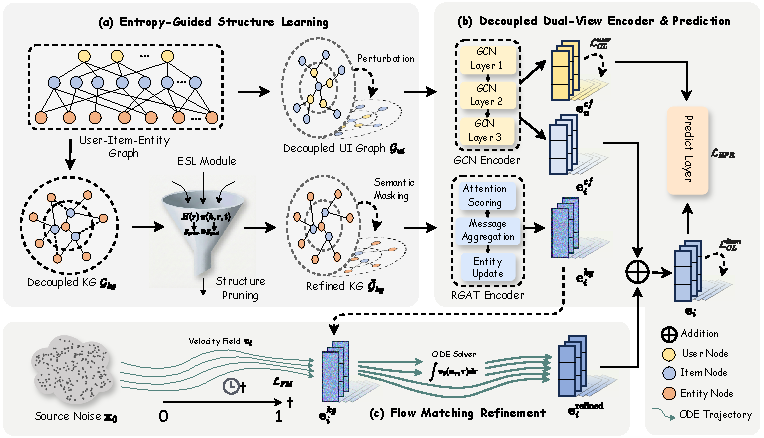
\includegraphics[width=\textwidth]{image/model2.pdf}
	\caption{Schematic overview of the proposed FlowKG framework. It incorporates an entropy-guided module for pre-filtering KG structure, a decoupled encoder for dual-view representation learning, and a flow matching module to refine latent embeddings via optimal transport paths.}
	\label{fig:model}
\end{figure*}


\subsection{Problem Formulation}
We model the task as link prediction within a heterogeneous information network.

\subsubsection{\textbf{User-Item Interaction Graph}}
Let $\mathcal{U}$ and $\mathcal{I}$ denote the sets of users and items, respectively. The historical interactions between users and items are represented as a bipartite graph $\mathcal{G}_{ui} = (\mathcal{U} \cup \mathcal{I}, \mathcal{E}_{ui})$, where each edge $(u, i) \in \mathcal{E}_{ui}$ indicates an observed interaction between user $u$ and item $i$.

\subsubsection{\textbf{Knowledge Graph (KG)}}
To incorporate auxiliary semantic information, we utilize a Knowledge Graph $\mathcal{G}_{kg} = (\mathcal{E}, \mathcal{R}, \mathcal{T})$, where $\mathcal{E}$, $\mathcal{R}$, and $\mathcal{T}$ represent the sets of entities, relations, and triplets, respectively. Items are mapped to corresponding entities within this graph, i.e., $\mathcal{I} \subseteq \mathcal{E}$. This mapping enriches the representation of items with contextual information, such as relations like (Movie, Director, Person).

\subsubsection{\textbf{Task Definition}}
Given $\mathcal{G}_{ui}$ and $\mathcal{G}_{kg}$, the objective is to learn a scoring function $\hat{y}_{ui} = f_\Theta(u, i)$ that predicts the likelihood of user $u$ interacting with an unobserved item $i$, generating a Top-$K$ ranking list. The goal is to generate a ranked list of Top-$K$ recommendations for each user.

\subsection{Flow Matching with Optimal Transport}
Flow Matching (FM) is a generative modeling framework grounded in the theory of Continuous Normalizing Flows (CNFs)~\cite{chen2018neural,grathwohl2018ffjord}. In contrast to diffusion models that rely on stochastic differential equations (SDEs)~\cite{ho2020denoising,song2020score}, FM constructs a deterministic probability path that transforms samples from a simple prior distribution $p_0$ (e.g., a Gaussian) into samples from the complex target data distribution $q(\mathbf{x})$.
The generative process is governed by an ordinary differential equation (ODE):
\begin{equation}
	\frac{\mathrm{d}\mathbf{x}_t}{\mathrm{d}t} = \mathbf{v}_t(\mathbf{x}_t; \theta), \quad t \in [0, 1],
\end{equation}
where $\mathbf{v}_t$ is a time-dependent vector field parameterized by a neural network. By numerically integrating this ODE, one can map an initial noise sample $\mathbf{x}_0 \sim p_0$ to a generated data sample $\mathbf{x}_1 \sim q(\mathbf{x})$.

To enable stable and efficient training, we adopt Conditional Flow Matching with Optimal Transport (OT) paths~\cite{tong2024improving}. An OT path corresponds to the straight-line interpolation between a source noise sample $\mathbf{x}_0$ and a target data sample $\mathbf{x}_1$, which minimizes the transport cost:
\begin{equation}
	\psi_t(\mathbf{x}_0, \mathbf{x}_1) = (1 - t)\mathbf{x}_0 + t \mathbf{x}_1.
\end{equation}
Differentiating this path with respect to time yields a simple, time-independent conditional vector field $\mathbf{u}_t$:
\begin{equation}
	\mathbf{u}_t(\mathbf{x} | \mathbf{x}_1) = \mathbf{x}_1 - \mathbf{x}_0.
\end{equation}
This implies that the learned model $\mathbf{v}t$ only needs to regress the constant displacement vector pointing from the noise to the target data sample. Consequently, the training objective simplifies to regressing this conditional vector field:
\begin{equation}
	\mathcal{L}_{\text{fm}}(\theta) = \mathbb{E}_{t, \mathbf{x}_0, \mathbf{x}_1} \left[ \| \mathbf{v}_t(\psi_t(\mathbf{x}_0, \mathbf{x}_1); \theta) - (\mathbf{x}_1 - \mathbf{x}_0) \|^2 \right].
	\label{eq:fm_loss}
\end{equation}
This straightforward and efficient formulation provides the mathematical basis for the representation refinement module in our framework.

%\subsection{\textbf{Problem Formulation}}
%We formulate the KG-enhanced recommendation task as a link prediction and ranking problem within a heterogeneous information network.
%
%\subsubsection{\textbf{User-Item Interaction Graph}}
%Let $\mathcal{U} = \{u_1, u_2, \dots, u_M\}$ denote the set of users and $\mathcal{I} = \{i_1, i_2, \dots, i_N\}$ denote the set of items, where $M$ and $N$ represent the number of users and items, respectively. The historical interaction data is constructed as a bipartite graph $\mathcal{G}_{ui} = (\mathcal{U} \cup \mathcal{I}, \mathcal{E}_{ui})$, where the edge set $\mathcal{E}_{ui}$ contains all observed interaction pairs $(u, i)$ (indicating implicit feedback $y_{ui}=1$).
%
%\subsubsection{\textbf{Knowledge Graph (KG)}}
%To incorporate external semantic information, we utilize a Knowledge Graph $\mathcal{G}_{kg} = (\mathcal{E}, \mathcal{R}, \mathcal{T})$. Here, $\mathcal{E}$ represents the set of entities, $\mathcal{R}$ is the set of relations, and $\mathcal{T} = \{(h, r, t) | h, t \in \mathcal{E}, r \in \mathcal{R}\}$ denotes the collection of triplets. In the recommendation scenario, the item set typically maps to a subset of the entity set, i.e., $\mathcal{I} \subseteq \mathcal{E}$. The KG provides rich semantic contexts for items (e.g., ``Movie-Director'' or ``Product-Brand'' associations).
%
%\subsubsection{\textbf{Task Definition}}
%Given the interaction graph $\mathcal{G}_{ui}$ and the knowledge graph $\mathcal{G}_{kg}$, our goal is to learn a scoring function $\hat{y}_{ui} = f_\Theta(u, i)$ to predict the preference probability of user $u$ for an unobserved item $i$. Based on these predicted scores, the system generates a Top-$K$ recommendation list sorted in descending order of preference for each user.
%
%\subsection{Flow Matching for Generative Modeling}
%Flow Matching (FM)~\cite{lipman2022flow} is a generative paradigm based on Continuous Normalizing Flows (CNF), designed to achieve distribution mapping by regressing a vector field along a fixed probability path. Compared to diffusion models, FM avoids complex Stochastic Differential Equation (SDE) simulations, offering more deterministic generation trajectories and more stable training objectives.
%
%\subsubsection{\textbf{Continuous Normalizing Flows via ODE}}
%FM models the sample generation process as a time-dependent probability density path $p_t(x)$ where $t \in [0, 1]$. This process is described by an Ordinary Differential Equation (ODE):
%\begin{equation}
%	\frac{\mathrm{d}x_t}{\mathrm{d}t} = v_t(x_t; \theta), \quad x_0 \sim p_0(x),
%\end{equation}
%where $x_t \in \mathbb{R}^d$ is the state vector, $v_t$ is the velocity vector field parameterized by a neural network, and $p_0$ is a known prior distribution (typically set as the standard Gaussian distribution $\mathcal{N}(0, \mathbf{I})$). By numerically integrating this ODE from $t=0$ to $t=1$, noise samples $x_0$ can be mapped to data samples $x_1$ that follow the target data distribution $p_1(x) \approx q(x)$.
%
%\subsubsection{\textbf{Conditional Flow Matching with Optimal Transport}}
%In practice, directly regressing the vector field of the marginal probability path is often intractable. Conditional Flow Matching (CFM) addresses this by introducing a conditional variable (i.e., the target data point $x_1$) to marginalize the vector field, thereby enabling efficient training without simulating ODE trajectories.
%
%Within the CFM framework, the **Optimal Transport (OT)** path has garnered significant attention due to its straight generation trajectories and minimal transport cost. The OT path is typically defined as a linear interpolation between the source noise $x_0$ and the target data $x_1$:
%\begin{equation}
%	\psi_t(x_0, x_1) = (1 - t)x_0 + t x_1.
%\end{equation}
%Differentiating this path with respect to time $t$ yields a constant closed-form solution for its corresponding conditional vector field:
%\begin{equation}
%	u_t(x | x_1) = x_1 - x_0.
%\end{equation}
%This concise form implies that the neural network $v_t$ only needs to learn to predict the ``displacement direction'' pointing from noise to data. Consequently, the training objective of FM simplifies to regressing this conditional vector field, with the loss function defined as:
%\begin{equation}
%	\mathcal{L}_{FM}(\theta) = \mathbb{E}_{t \sim \mathcal{U}[0,1], x_0 \sim p_0, x_1 \sim q(x)} \left[ \| v_t(\psi_t(x_0, x_1); \theta) - (x_1 - x_0) \|^2 \right].
%	\label{eq:fm_loss}
%\end{equation}
%During the inference phase, given an initial noise $x_0$, the model reconstructs the data representation by advancing along the learned vector field using a numerical solver (e.g., the Euler method).

\section{Methodology}
\label{sec:method}
% !TEX spellcheck = en_US
% !TeX root = main.tex




%This section presents FlowKG, a novel framework designed to address structural noise and representation degradation in knowledge graph-enhanced recommendation through three synergistic components, as illustrated in Figure~\ref{fig:model}.

In this section, we introduce FlowKG, a novel framework designed to combat structural noise and representation degradation in knowledge graph-enhanced recommendation. FlowKG comprises three synergistic components, as illustrated in Figure~\ref{fig:model}: an Entropy-Guided Structure Learning (ESL) module, a Decoupled Dual-View Encoder, and a Flow Matching Representation Refinement module.

\subsection{Overall Architecture}
Our framework operates through three interconnected stages designed to sequentially address the core challenges.
First, to mitigate the pervasive noisy connections within real-world KGs, we propose the Entropy-Guided Structure Learning (ESL) module. This module adaptively prunes low-informative triplets by integrating a static relational entropy prior with a dynamic, learnable semantic posterior, yielding a refined and task-relevant graph structure.
Second, the refined KG and the user-item interaction graph are processed in parallel by the Decoupled Dual-View Encoder. This design explicitly severs the direct propagation of KG noise into the collaborative signal space, capturing complementary signals from the two views while constructing robust augmented representations for contrastive learning. Finally, to counteract the over-smoothing effect inherent in multi-layer GNNs and to further purify residual noise, we introduce the Flow Matching Refinement module. It models the evolution of item embeddings as a continuous trajectory defined by an ODE, transforming potentially noisy or sub-optimal representations into a refined semantic manifold.
%Our framework operates through three mutually reinforcing stages. First, to mitigate the prevalent noisy connections in KGs, we propose the Entropy-Guided Structure Learning (ESL) module. This module adaptively prunes low-quality triplets by integrating a static entropy prior with a dynamic semantic posterior. Second, the refined graph, along with the user-item interaction graph, is fed into the Decoupled Dual-View Encoder. This encoder captures collaborative and semantic signals in parallel and explicitly constructs augmented views to facilitate CL. Finally, to combat the over-smoothing effect inherent in GNNs, we introduce the Flow Matching Refinement module, which models embedding evolution as continuous ODEs, transforming noisy representations into robust target distributions.

\subsection{Entropy-Guided Structure Learning}
In real-world KGs, relations exhibit significant variance in their informativeness. We posit that relations crucial for recommendation often demonstrate high specificity (i.e., low uncertainty), whereas overly generalized relations manifest high structural uncertainty (or ``entropy"). High entropy can signal potential noise but does not guarantee it; some such triplets may still carry valuable semantics. For example, the relation `Movie $\rightarrow$ directed\_by $\rightarrow$ Nolan' is typically unique, conveying a strong stylistic signal. In contrast, relations like `Movie $\rightarrow$ starring $\rightarrow$ \{Actor List\}' or `Item $\rightarrow$ also\_bought $\rightarrow$ \{Massive Items\}' connect a head entity to a vast, diverse set of tails, introducing high uncertainty and potential semantic drift during aggregation. To address this, we design a structure learning mechanism that fuses a static entropy prior with a dynamic semantic posterior.


\subsubsection{Relation Entropy Prior}

To estimate the structural reliability of different relations, we compute a relation-level branching entropy for each relation \(r \in \mathcal{R}\). Intuitively, if a relation frequently connects a head entity to many tail entities, it usually exhibits weaker structural specificity and higher uncertainty, and may therefore introduce more noisy or less informative semantic signals. In contrast, relations with nearly one-to-one or one-to-few patterns tend to provide stronger structural constraints and should be assigned higher prior confidence.

Formally, for a given relation \(r\), let \(\mathcal{N}_{h}^{r}\) denote the tail entities connected to head entity \(h\) through \(r\), and let \(\mathcal{H}_{r}\) denote all head entities associated with relation \(r\). Following the derivation in Appendix~\ref{app:relation_entropy}, we define the structural uncertainty of relation \(r\) as the average branching entropy over its associated head entities:
\begin{equation}
\label{eq:relation_branching_entropy}
H(r)
=
\frac{1}{|\mathcal{H}_{r}|}
\sum_{h\in \mathcal{H}_{r}}
\log |\mathcal{N}_{h}^{r}|.
\end{equation}

A larger \(H(r)\) indicates that relation \(r\) tends to connect each head entity to more tail entities on average, implying higher structural dispersion and weaker relation specificity. We then convert this entropy into a normalized inverse-entropy prior:
\begin{equation}
\label{eq:relation_entropy_prior}
S_{\mathrm{prior}}(r)
=
1-\frac{H(r)}{\max_{r'\in\mathcal{R}}H(r')}.
\end{equation}

Therefore, relations with lower branching entropy obtain higher structural prior scores and are more likely to be preserved during triplet filtering, while relations with higher branching entropy are treated more conservatively. This design allows the model to suppress potentially noisy or weakly specific relations before triplet-level semantic scoring.

\subsubsection{\textbf{Semantic Posterior Scoring}}


While the entropy prior provides valuable global guidance, it operates at the relation level and may overlook the semantic importance of individual triplets. For instance, even within a high-entropy relation like ``also\_bought'', certain specific item pairs may convey strong co-preference signals. To capture such instance-level nuances, we introduce a learnable posterior based on a relational graph attention mechanism.

%While the structural prior offers valuable global guidance, it operates at the relation level and may overlook the semantic importance of individual triplets. For instance, even within a high-entropy relation like ``also\_bought'', certain specific connections may still convey strong preference signals. To capture such nuances, we introduce a learnable posterior that evaluates each triplet $(h, r, t)$ individually via a relational graph attention mechanism.

Given entity embeddings $\mathbf{e}_h, \mathbf{e}_t \in \mathbb{R}^d$ and relation embedding $\mathbf{e}_r \in \mathbb{R}^d$, where $d$ is the embedding dimension, we compute a compatibility score via a learnable transformation $\mathbf{W}_g \in \mathbb{R}^{d \times 2d}$:
\begin{equation}
	\label{eq:triplet_score}
	\pi(h, r, t) = \left( \mathbf{W}_g [\mathbf{e}_h \| \mathbf{e}_t] \right)^\top \mathbf{e}_r,
\end{equation}
where $[\cdot \| \cdot]$ denotes concatenation. The posterior score is obtained by applying a non-linear activation followed by normalization:
\begin{equation}
	S_{\text{post}}(h, r, t) = \text{Norm} \left( \text{LeakyReLU}(\pi(h, r, t)) \right),
\end{equation}
where $\text{Norm}(\cdot)$ is a normalization function (e.g., Sigmoid) that maps the score to $(0,1)$. This score dynamically captures the semantic plausibility of the triplet under the current model parameters.

\subsubsection{\textbf{Adaptive Structure Pruning}}
At the start of each training epoch, we fuse the prior and posterior scores to obtain a comprehensive quality assessment for each triplet:
\begin{equation}
	S_{\text{final}}(h, r, t) = (1 - \alpha) \cdot S_{\text{prior}}(r) + \alpha \cdot S_{\text{post}}(h, r, t),
\end{equation}
where $\alpha \in [0,1]$ is a balancing coefficient. This design treats the entropy prior as soft guidance rather than a hard filter---triplets from high-entropy relations can still survive if their learned semantic score is high, preventing the indiscriminate removal of valuable connections. To flexibly control the filtering intensity, we adopt a ratio-based retention strategy. Given a retention rate hyperparameter $\rho \in (0, 1]$, we sort all triplets in descending order based on $S_{\text{final}}$ and retain only the top $K = \lfloor \rho \cdot |\mathcal{G}_{kg}| \rfloor$ triplets to form the refined graph $\tilde{\mathcal{G}}_{kg}$:
\begin{equation}
\tilde{\mathcal{G}}_{kg} = \text{TopK}(\mathcal{G}_{kg}, K).
\end{equation}
This adaptive mechanism reinforces task-relevant connections based on integrated scores, providing a high-quality graph foundation for subsequent representation learning.

\subsection{Decoupled Dual-View Encoder}
To prevent structural noise from the KG from contaminating collaborative signals—a common issue in cascaded architectures—we propose a Decoupled Dual-View Encoder. This module processes the User-Item (UI) graph and the refined KG in parallel, extracting complementary signals while maintaining explicit isolation between the two representation spaces.

We maintain two embedding tables: user embeddings $\mathbf{E}_u \in \mathbb{R}^{|\mathcal{U}| \times d}$ and  entity embeddings $\mathbf{E}_e \in \mathbb{R}^{|\mathcal{E}| \times d}$. Since items are a subset of entities ($\mathcal{I} \subseteq \mathcal{E}$), item embeddings are  indexed directly from $\mathbf{E}_e$, ensuring semantic consistency across both views.

\subsubsection{\textbf{Collaborative View Encoder}}
We employ a LightGCN~\cite{he2020lightgcn} backbone to capture collaborative signals on $\mathcal{G}_{ui}$. The propagation at layer $l$ is defined as:
\begin{equation}
	\mathbf{e}_u^{(l)} = \sum_{i \in \mathcal{N}_u} \frac{\mathbf{e}_i^{(l-1)}}{\sqrt{|\mathcal{N}_u| |\mathcal{N}_i|}}, \quad \mathbf{e}_i^{(l)} = \sum_{u \in \mathcal{N}_i} \frac{\mathbf{e}_u^{(l-1)}}{\sqrt{|\mathcal{N}_i| |\mathcal{N}_u|}},
\end{equation}
where $\mathcal{N}_u$ and $\mathcal{N}_i$ denote the neighbor sets in $\mathcal{G}_{ui}$. After $L_{cf}$ layers, we obtain the collaborative representation $\mathbf{e}^{cf}$.

For contrastive augmentation, we adopt Sign-Preserving Noise Perturbation inspired by SimGCL~\cite{yu2022graph}. Instead of risky edge-dropping on sparse graphs, this method injects controlled noise directly into the embedding space while preserving the sign of original vectors to maintain semantic consistency:
\begin{equation}
	\mathbf{E}^{(l)}_{\text{aug}} = \tilde{\mathbf{A}}_{ui} \left( \mathbf{E}^{(l-1)} + \epsilon \cdot \text{sign}(\mathbf{E}^{(l-1)}) \odot \boldsymbol{\Delta} \right),
\end{equation}
where $\tilde{\mathbf{A}}_{ui}$ is the symmetrically normalized adjacency matrix of $\mathcal{G}_{ui}$, $\boldsymbol{\Delta} \sim \mathcal{U}(0, 1)$ denotes a uniform noise matrix, and $\epsilon$ controls the perturbation magnitude. This yields the augmented view $\tilde{\mathbf{e}}^{cf}$ for robust alignment.

\subsubsection{\textbf{Semantic View Encoder}}
To capture high-order attributes, we deploy a Relational Graph Attention Network (RGAT)~\cite{yang2022knowledge,wang2019kgat} on the refined graph $\tilde{\mathcal{G}}_{kg}$ (from ESL). Starting from  $\mathbf{E}_e$, attention coefficients $\alpha_{hrt}^{(l)}$ are derived by normalizing the compatibility scores $\pi(h, r, t)$ (Eq.~\eqref{eq:triplet_score}) via softmax.
Entity representations are recursively updated by aggregating neighbor information:
\begin{equation}
	\mathbf{e}_h^{(l)} = \mathbf{e}_h^{(l-1)} + \sum\nolimits_{(h,r,t) \in \tilde{\mathcal{G}}_{kg}} \alpha_{hrt}^{(l)} \cdot \mathbf{e}_t^{(l-1)}.
\end{equation}
Stacking $L_{kg}$ layers yields the semantic representation $\mathbf{e}^{kg}$.

For augmentation, we propose Stochastic Semantic Masking (SSM). To avoid breaking critical sparse connections via edge dropping, SSM perturbs the information flow in the latent space by applying a Bernoulli mask $\mathbf{M}^{(l)} \sim \text{Bernoulli}(1-p)$ to aggregated features, where $p$ denotes the dropout probability:
\begin{equation}
	\tilde{\mathbf{e}}_h^{(l)} = \mathbf{e}_h^{(l-1)} + \left( \sum_{(h,r,t) \in \tilde{\mathcal{G}}_{kg}} \alpha_{hrt}^{(l)} \cdot \mathbf{e}_t^{(l-1)} \right) \odot \mathbf{M}^{(l)}.
\end{equation}
This forces the model to reconstruct semantics from partial cues, producing the augmented view $\tilde{\mathbf{e}}^{kg}$ robust to specific noise patterns.
\subsection{Flow Matching Representation Refinement}
Despite the preceding modules, item embeddings may still suffer from residual noise or sub-optimal positioning due to GNN over-smoothing and KG sparsity. We address this by reframing representation learning as a continuous denoising and refinement process. Inspired by Flow Matching (FM)~\cite{lipman2023flow}, we model the evolution from a simple noise distribution to a target high-quality embedding distribution via a deterministic ODE, offering superior stability and efficiency compared to diffusion models.

%Despite the effective feature extraction by entropy-guided structure learning and the dual-view encoder, the inevitable over-smoothing issue in graph convolution and the inherent long-tail distribution of KGs may still render the final item embeddings susceptible to latent noise or leave them in a sub-optimal representation space. We address this issue by modeling item representation refinement as a continuous dynamic evolution process from a simple noise distribution to a high-quality semantic distribution.
%
%Inspired by recent advances in generative modeling, we introduce FM~\cite{lipman2023flow}. Unlike diffusion models based on SDEs, FM constructs generation trajectories via deterministic ODEs, offering superior training stability and inference efficiency.

\subsubsection{\textbf{Optimal Transport Path Construction}}
We instantiate a Conditional Flow Matching framework based on OT. During training, we pair a source noise sample \(\mathbf{x}_0 \sim \mathcal{N}(\mathbf{0}, \mathbf{I})\) with a target semantic embedding \(\mathbf{x}_1 = \mathbf{e}_i^{kg}\). The OT path defines a straight-line interpolation and its corresponding conditional vector field:
\begin{equation}
	\mathbf{x}_t = (1 - t)\mathbf{x}_0 + t\mathbf{x}_1, \quad \mathbf{u}_t(\mathbf{x}_t | \mathbf{x}_1) = \mathbf{x}_1 - \mathbf{x}_0,
\end{equation}
for \(t \in [0,1]\). This simplifies the learning target to a constant displacement vector pointing from noise to the semantic proxy.

\subsubsection{\textbf{Vector Field Estimator and Training}}
To approximate the ideal vector field, we introduce a parameterized neural network $\text{FlowNet}$, denoted as $\mathbf{v}_t(\mathbf{x}; \theta)$, where $\theta$ represents the network parameters. To incorporate temporal information, we first map the scalar time step $t$ to a high-dimensional time embedding $\mathbf{t}_{\text{emb}}$ via sinusoidal positional encoding and MLP projection. Then, we concatenate this time vector with the current noisy state $\mathbf{x}_t$ and feed the result into an MLP to predict the velocity field:
\begin{equation}
	\mathbf{v}_t(\mathbf{x}_t; \theta) = \text{MLP}([\mathbf{x}_t \| \mathbf{t}_{\text{emb}}]; \theta).
\end{equation}
The model is trained to regress the true displacement using the Conditional Flow Matching loss:
\begin{equation}
	\mathcal{L}_{\text{fm}} = \mathbb{E}_{t, \mathbf{x}_0, \mathbf{x}_1} \left[ \| \mathbf{v}_t(\mathbf{x}_t; \theta) - (\mathbf{x}_1 - \mathbf{x}_0) \|^2 \right].
\end{equation}

\subsubsection{\textbf{Euler Integration Strategy}}
A key insight of our approach is the dual role of $\mathbf{e}_i^{kg}$: during training, it serves as the target state $\mathbf{x}_1$ to supervise the vector field; during inference, it is re-interpreted as an intermediate state $\mathbf{x}_{t_{\text{start}}}$ on the OT path. This design is motivated by the observation that while $\mathbf{e}_i^{kg}$ captures useful semantics, it may still contain residual noise from the KG. By treating it as a ``partially evolved'' state rather than the final destination, we allow the learned vector field to further refine it toward a higher-quality manifold.

Concretely, we set the initial condition as $\mathbf{x}_{t_{\text{start}}} = \mathbf{e}_i^{kg}$ and integrate from $t_{\text{start}}$ to $t=1$ using the Euler Method. Discretizing this interval into $N$ steps, the update rule is:
\begin{equation}
	\mathbf{x}_{t_{n+1}} = \mathbf{x}_{t_n} + \mathbf{v}_{t_n}(\mathbf{x}_{t_n}; \theta) \cdot (t_{n+1} - t_n).
\end{equation}
To balance computational cost and refinement quality, we adopt an adaptive step strategy: during training, we set $N=1$ for single-step refinement to ensure efficient gradient backpropagation; during inference, we can flexibly increase $N$ to obtain a finer manifold evolution trajectory. The final $\mathbf{x}_1$ obtained at time $t=1$ serves as the refined semantic representation $\mathbf{e}_i^{\text{refined}}$.

\subsection{Prediction and Optimization}

\subsubsection{\textbf{Representation Fusion and Prediction}}
To integrate the generative refinement into the recommendation task, we fuse the collaborative embedding $\mathbf{e}_i^{cf}$ and the flow-refined semantic embedding $\mathbf{e}_i^{\text{refined}}$ (computed via a single Euler step $N=1$ for efficient gradient feedback) via summation: $\mathbf{e}_i = \mathbf{e}_i^{cf} + \mathbf{e}_i^{\text{refined}}$.
The user preference score is calculated as the inner product $\hat{y}_{ui} = {\mathbf{e}_u^{cf}}^\top \mathbf{e}_i$.
We employ the Bayesian Personalized Ranking (BPR) loss~\cite{rendle2012bpr} as the primary objective to maximize the margin between observed and unobserved interactions:
\begin{equation}
	\mathcal{L}_{\text{BPR}} = - \sum\nolimits_{(u, i, j) \in \mathcal{D}} \ln \sigma(\hat{y}_{ui} - \hat{y}_{uj}),
\end{equation}
where $\mathcal{D}$ denotes the training set of triplets $(u, i, j)$, with $i$ being the observed item and $j$ being the sampled negative item.

\subsubsection{\textbf{Dual-Level Contrastive Learning}}
To enhance robustness, we perform contrastive learning on both user and item views.
For users, we align $\mathbf{e}_u^{cf}$ with its augmented view $\tilde{\mathbf{e}}_u^{cf}$; for items, we align the fused embedding $\mathbf{e}_i$ with its flow-augmented counterpart $\tilde{\mathbf{e}}_i$.  
We adopt the InfoNCE loss~\cite{oord2018representation} to maximize the mutual information of positive pairs:
\begin{equation}
	\mathcal{L}_{\text{cl}} = - \sum\nolimits_{x \in \mathcal{B}} \ln \frac{\exp(\text{sim}(\mathbf{e}_x, \tilde{\mathbf{e}}_x) / \tau)}{\sum_{y \in \mathcal{B}} \exp(\text{sim}(\mathbf{e}_x, \tilde{\mathbf{e}}_y) / \tau)},
\end{equation}
where $\mathcal{B}$ denotes the batch, $\text{sim}(\cdot, \cdot)$ is cosine similarity, and $\tau$ is temperature. We analyze the asymptotic behavior as \(\tau \to \infty\), where the objective converges to a Mean Difference (MD) loss~\cite{wang2021understanding}:
\begin{equation}
	\label{eq:md_loss}
	\mathcal{L}_{\text{md}} \propto \mathbb{E}_{x \in \mathcal{B}} \left[ \mathbb{E}_{y \in \mathcal{B}} [\text{sim}(\mathbf{e}_x, \tilde{\mathbf{e}}_y)] - \text{sim}(\mathbf{e}_x, \tilde{\mathbf{e}}_x) \right].
\end{equation}
As evidenced in ~\cite{wang2021understanding}, this global alignment strategy is theoretically more robust against false negatives in sparse data scenarios.

\subsubsection{\textbf{Multi-Task Objective}}
The final objective jointly optimizes recommendation, generation, and self-supervised alignment:
\begin{equation}
	\mathcal{L} = \mathcal{L}_{\text{BPR}} + \lambda_{\text{fm}} \mathcal{L}_{\text{fm}} + \lambda_{u} \mathcal{L}_{\text{cl}}^u + \lambda_{i} \mathcal{L}_{\text{cl}}^i + \lambda_{\text{reg}} \|\Theta\|_2^2,
\end{equation}
where $\Theta$ denotes all learnable parameters (including $\theta$ in FlowNet), and $\lambda_{u}$, $\lambda_{i}$, $\lambda_{\text{fm}}$, $\lambda_{\text{reg}}$ are  balancing hyperparameters. During inference, we discard the contrastive branch and utilize the trained FlowNet with flexible steps for high-quality refinement.




%\newpage
%\subsection{Decoupled Dual-View Encoder}
%Conventional knowledge-aware recommendation methods typically rely on \textit{cascaded architectures}, where item embeddings are first enriched via KG aggregation and subsequently propagated through the user-item graph. However, this tight coupling inevitably propagates and amplifies inherent structural noise from the KG into the collaborative signal, thereby degrading recommendation performance. To address this, we propose a Decoupled Dual-View Encoder. This module processes the user-item interaction graph (Collaborative View) and the knowledge graph (Semantic View) in parallel, extracting complementary representations while strictly insulating the collaborative learning process from direct KG noise interference.
%
%\subsubsection{\textbf{Collaborative View Encoder}}
%The collaborative view is designed to capture high-order collaborative signals from the user-item bipartite graph $\mathcal{G}_{ui}$. Following the minimalist design of LightGCN~\cite{he2020lightgcn}, we employ a lightweight graph convolutional network (GCN) as the backbone, removing burdensome feature transformations and non-linear activations.
%Crucially, to prevent potential KG noise from contaminating the collaborative space, we initialize item features with independent ID embeddings $\mathbf{E}^{(0)} \in \mathbb{R}^{N \times d}$ rather than reusing KG-derived embeddings. We perform standard graph convolution to generate the base view. At the $l$-th layer, the user and item embeddings are updated as follows:
%\begin{equation}
%	\mathbf{e}_u^{(l)} = \sum_{i \in \mathcal{N}_u} \frac{\mathbf{e}_i^{(l-1)}}{\sqrt{|\mathcal{N}_u| |\mathcal{N}_i|}}, \quad \mathbf{e}_i^{(l)} = \sum_{u \in \mathcal{N}_i} \frac{\mathbf{e}_u^{(l-1)}}{\sqrt{|\mathcal{N}_i| |\mathcal{N}_u|}},
%\end{equation}
%where $\mathcal{N}_u$ and $\mathcal{N}_i$ denote the neighbor sets of user $u$ and item $i$, respectively. After stacking $L_{cf}$ propagation layers, we obtain the final collaborative representations, denoted as $\mathbf{e}^{cf} = \mathbf{e}^{(L_{cf})}$.
%
%To construct the augmented view for contrastive learning, we introduce a controlled noise perturbation strategy. Unlike structural perturbations (e.g., edge dropout) that may fracture sparse interaction graphs, embedding-level noise injection offers greater efficiency and stability. To preserve semantic consistency, we constrain the noise to strictly maintain the sign of the original embeddings, ensuring the augmented vectors remain within the same hyper-quadrant. Specifically, at each layer, the augmented representation is computed as:
%\begin{equation}
%	\mathbf{E}^{(l)}_{\text{aug}} = \tilde{\mathbf{A}}_{ui} \left( \mathbf{E}^{(l-1)} + \epsilon \cdot \text{sign}(\mathbf{E}^{(l-1)}) \odot \Delta \right),
%\end{equation}
%where $\Delta \sim \mathcal{U}(0, 1)^{N \times d}$ is a uniform random noise matrix, $\epsilon$ controls the perturbation magnitude, and $\odot$ is the Hadamard product. This strategy introduces necessary variance for contrastive alignment while preserving the integrity of the collaborative signals, yielding the augmented view $\tilde{\mathbf{e}}^{cf}$.
%
%\subsubsection{\textbf{Semantic View Encoder}}
%The semantic view focuses on extracting high-order attribute features by propagating information over the refined knowledge graph $\tilde{\mathcal{G}}_{kg}$ (produced by the ESL module). To capture deep semantic dependencies beyond immediate neighbors, we employ a Relational Graph Attention Network (RGAT).
%
%Analogous to the collaborative view, we perform recursive embedding propagation. We initialize entity representations as $\mathbf{e}_h^{(0)} = \mathbf{e}_h$. At the $l$-th layer, we first compute the normalized attention coefficients for each triplet $(h, r, t) \in \tilde{\mathcal{G}}_{kg}$ utilizing the compatibility score $\pi(h, r, t)$ (defined in Section 3.2.2):
%\begin{equation}
%	\alpha_{hrt}^{(l)} = \frac{\exp(\text{LeakyReLU}(\pi(h, r, t)))}{\sum_{t' \in \mathcal{N}_h^r} \exp(\text{LeakyReLU}(\pi(h, r, t')))},
%\end{equation}
%where $\mathcal{N}_h^r$ denotes the set of tail entities connected to head entity $h$ via relation $r$. Subsequently, we aggregate the neighbor information from the $(l-1)$-th layer to update the head entity representation:
%\begin{equation}
%	\mathbf{e}_h^{(l)} = \mathbf{e}_h^{(l-1)} + \sum_{(h,r,t) \in \tilde{\mathcal{G}}_{kg}} \alpha_{hrt}^{(l)} \cdot \mathbf{e}_t^{(l-1)}.
%\end{equation}
%After performing $L_{kg}$ layers of recursive propagation, we obtain the final semantic representation, denoted as $\mathbf{e}^{kg} = \mathbf{e}^{(L_{kg})}$, which encodes the comprehensive high-order semantic context.
%
%For the augmented semantic view, we propose a Stochastic Semantic Masking (SSM) strategy. Considering that dropping edges in a sparse KG might sever critical semantic connections, SSM perturbs the information flow directly in the latent space while keeping the topology intact. During aggregation at the $l$-th layer, we introduce a Bernoulli mask $\mathcal{M}^{(l)} \sim \text{Bernoulli}(1-p)$ to randomly drop dimensions of the aggregated features:
%\begin{equation}
%	\tilde{\mathbf{e}}_h^{(l)} = \mathbf{e}_h^{(l-1)} + \left( \sum_{(h,r,t) \in \tilde{\mathcal{G}}_{kg}} \alpha_{hrt}^{(l)} \cdot \mathbf{e}_t^{(l-1)} \right) \odot \mathcal{M}^{(l)}.
%\end{equation}
%This process yields the augmented semantic representation $\tilde{\mathbf{e}}^{kg}$. By compelling the model to reconstruct representations from partial semantic cues, SSM effectively prevents overfitting to specific noise patterns and enhances the robustness of the learned entity embeddings.

\section{Experiment}
\label{sec:experiment}
% !TEX spellcheck = en_US
% !TeX root = main.tex


\noindent Extensive experiments are performed to evaluate the performance of our FlowKG by answering the following research questions:

\begin{itemize}
	\item \textbf{RQ1:} How does FlowKG perform compared to state-of-the-art recommendation baselines?
	\item \textbf{RQ2:} How do key components contribute to the model's effectiveness, and how do critical hyperparameters influence its performance?
	\item \textbf{RQ3:} Can FlowKG effectively mitigate the impact of knowledge noise and maintain robustness across varying data distributions?
	\item \textbf{RQ4:} How does the computational efficiency (in terms of training time and model parameters) of FlowKG compare to state-of-the-art baselines?
	\item \textbf{RQ5:} Can the learned representations visually demonstrate the manifold refinement process and semantic separation of items?
\end{itemize}

\subsection{Experimental Settings}

\subsubsection{\textbf{Datasets}}
To ensure comprehensive evaluation across diverse domains and sparsity levels, we utilize four benchmark datasets: MIND~\cite{wu2020mind} (News), MovieLens-1M~\cite{harper2015movielens} (Movies), Last-FM~\cite{cantador2011second} (Music), and Yelp\footnote{\url{https://www.yelp.com/dataset}} (Business). To guarantee data quality and fairness, we employ a unified KG construction approach and apply a 10-core filtering setting~\cite{jiang2024diffkg,li2025mask}. Consistent with standard protocols, we adopt an 80:10:10 split for training, validation, and testing, respectively. Table~\ref{tab:data statistics} summarizes the detailed statistics of the User-Item Graphs and Knowledge Graphs for all datasets.

\subsubsection{\textbf{Evaluation Protocols}}
We implement a comprehensive all-ranking strategy~\cite{ren2024representation,wang2019kgat,yang2023knowledge} to evaluate recommendation performance. To strictly assess the quality of Top-$N$ recommendations, we employ two widely adopted metrics: Recall@20 and NDCG@20. Recall measures the proportion of relevant items successfully retrieved, while NDCG evaluates the ranking quality by assigning higher scores to hits positioned near the top of the list.

\subsubsection{\textbf{Baselines for Comparison}}
To benchmark the effectiveness of FlowKG, we compare it against a diverse set of state-of-the-art knowledge-aware recommenders.

\noindent\textbf{Conventional Embedding and Translation-based Methods.}
\begin{itemize}
	\item \textbf{FM}~\cite{rendle2011fast} is a classic embedding-based method that models high-order feature interactions via factorized parameters to incorporate context information as auxiliary features.
	\item \textbf{CKE}~\cite{zhang2016collaborative} integrates collaborative filtering with structural, textual, and visual knowledge embeddings extracted via TransR and auto-encoders.
	\item \textbf{KTUP}~\cite{cao2019unifying} employs a translation-based approach to jointly learn recommendation and knowledge graph completion tasks, transferring relational information to model user preferences.
\end{itemize}

\noindent\textbf{Propagation-based Graph Neural Network Methods.}
\begin{itemize}
	\item \textbf{KGAT}~\cite{wang2019kgat} applies graph neural networks with an attention mechanism to recursively propagate embeddings and model high-order connectivities within a collaborative knowledge graph.
	\item \textbf{KGIN}~\cite{wang2021learning} explores latent user intents behind interactions by aggregating relational paths and modeling intents as attentive combinations of KG relations.
	\item \textbf{LECF}~\cite{huang2024lorentz} leverages hyperbolic geometry to capture hierarchical structures in knowledge graphs and ensures Lorentz group equivariance during the message propagation process.
\end{itemize}


\setlength{\tabcolsep}{3pt}
\begin{table}[t]
	\small
	\centering
	\caption{Statistics of the experimental datasets.}
	\label{tab:data statistics}
		\begin{tabular}{lrrrr}
			\toprule
			Statistics & MIND & ML-1M & Last-FM & Yelp \\
			\midrule
			\# Users & 100,000 & 6,036 & 1,815 & 16,308 \\
			\# Items & 30,577 & 2,347 & 3,846 & 11,516 \\
			\# Interactions & 2,975,319 & 301,509 & 17,523 & 159,302 \\
			\midrule
			\multicolumn{5}{c}{Knowledge Graph} \\
			\midrule
			\# Entities & 49,545 & 6,729 & 9,366 & 24,176 \\
			\# Relations & 512 & 12 & 60 & 42 \\
			\# Triples & 297,058 & 38,346 & 19,586 & 47,204 \\
			\bottomrule
		\end{tabular}
\end{table}

\noindent\textbf{Self-Supervised Contrastive Learning Frameworks.}
\begin{itemize}
	\item \textbf{KGIC}~\cite{zou2022improving} introduces a multi-level interactive contrastive learning mechanism that contrasts local and non-local graph views to mitigate data sparsity and noise.
	\item \textbf{KGRec}~\cite{yang2023knowledge} proposes a self-supervised rationalization framework that identifies informative knowledge connections through generative masking and contrastive alignment tasks.
	\item \textbf{LightKG}~\cite{li2025lightkg} features a simplified GNN architecture with linear aggregation and an efficient contrastive layer to address data sparsity and computational complexity.
\end{itemize}

\noindent\textbf{Generative and Diffusion-based Recommendation Models.}
\begin{itemize}
	\item \textbf{DiffKG}~\cite{jiang2024diffkg} integrates a generative diffusion model with data augmentation to reconstruct the knowledge graph and align semantic signals with collaborative data.
	\item \textbf{KMDCL}~\cite{li2025mask} combines mask-based diffusion models with contrastive learning to adaptively generate denoised views guided by user intentions for robust representation learning.
\end{itemize}


%\subsubsection{\textbf{Parameter Settings.}}
%Our baseline settings are consistent with our model parameter configurations, and any additional parameters for baselines follow the default settings reported in their respective papers or public implementations.
%We employ a fixed learning rate of $1e^{-4}$, a batch size of 1024, and a fixed embedding dimension of 64. The FlowKG framework was optimized using the Adam optimizer, with model parameters initialized via Xavier initialization.
%
%Regarding the model-specific hyperparameters, we conducted a grid search to identify optimal configurations.
%\begin{itemize}
%	\item \textbf{Dual-View Encoder:} The number of layers for the collaborative view ($L_{cf}$) and the semantic view ($L_{kg}$) are tuned independently within the range of $\{1, 2, 3\}$. The noise perturbation magnitude $\epsilon$ is searched in $\{0.05, 0.1, 0.2, 0.5\}$.
%	\item \textbf{Structure Learning:} For the entropy-guided structure learning module, both the retention rate $\rho$ and the balance factor $\alpha$ are tuned in the range of $\{0.1, 0.2, \dots, 0.9\}$.
%	\item \textbf{Flow Matching:} The time step embedding size is fixed to 10. The starting time step of the evolution trajectory, denoted as $t_{\text{start}}$, is tuned in the range of $\{0.1, 0.2, \dots, 0.9\}$. Regarding the Euler integration strategy, we explore the integration steps $N$ in the range of $\{1, \dots, 5\}$ during the inference phase to balance efficiency and performance.
%	\item \textbf{Loss and Regularization:} The contrastive loss weight $\lambda_1$ is optimized in $\{0.0, 0.2, \dots, 1.0\}$, and the flow matching loss weight $\lambda_2$ is tuned in $\{1, 2, 5, 10, 20\}$. The temperature hyperparameter $\tau$ is searched in $\{0.1, 0.2, \dots, 1.0\}$. Notably, for datasets exhibiting a preference for higher temperatures, we further investigate the asymptotic limit where $\tau \to \infty$, implemented as the Mean Difference (MD) loss, to evaluate the effectiveness of global alignment in the representation space. The $L_2$ regularization coefficient $\lambda_{reg}$ is searched in $\{1e^{-7}, 1e^{-6}, 1e^{-5}\}$.
%\end{itemize}
%These parameter configurations establish an initial tuning baseline, which is further refined based on the validation performance. We implemented our model using PyTorch on an NVIDIA RTX 4090 GPU.
%\begin{table}[t]
%	\centering
%	\caption{Statistics of the experimental datasets.}
%	\label{tab:data statistics}
%	\renewcommand{\arraystretch}{1.2}
%	\setlength{\tabcolsep}{2pt}
%	\begin{tabular}{lcccc}
	%		\toprule
	%		Statistics & MIND & MovieLens-1M & Last-FM & Yelp \\
	%		\midrule
	%		Users        & 100,000 & 6,036 & 1,815 & 16,308 \\
	%		Items        & 30,577  & 2,347 & 3,846 & 11,516 \\
	%		Interactions & 2,975,319 & 301,509 & 17,523 & 159,302 \\
	%		\midrule
	%		Entities     & 49,545 & 6,729 & 9,366 & 24,176 \\
	%		Relations    & 512    & 12    & 60    & 42 \\
	%		KG triples   & 297,058 & 38,346 & 19,586 & 47,204 \\
	%		\bottomrule
	%	\end{tabular}
%\end{table}


\subsubsection{\textbf{Parameter Settings}}
We implement FlowKG and all baselines using PyTorch on an NVIDIA RTX 4090 GPU. For a fair comparison, we fix the embedding dimension to 64, the batch size to 1024, and the learning rate to $1e^{-4}$, optimizing the model via Adam~\cite{kingma2014adam} with Xavier initialization~\cite{xavier2007unravelling}. Baseline hyperparameters follow the optimal settings reported in their respective papers. For FlowKG, we determine the optimal hyperparameters via grid search on the validation set. Specifically, the layer depths for collaborative and semantic views ($L_{cf}, L_{kg}$) are tuned in $\{1, 2, 3\}$, and the noise perturbation $\epsilon$ is searched in $\{0.05, \dots, 0.5\}$. The structure learning parameters $\rho$ and $\alpha$ are adjusted within $[0.1, 0.9]$. For the Flow Matching module, we set the time step embedding size to 10 and tune the start time $t_{\text{start}}$ in $[0.1, 0.9]$. Regarding the optimization objectives, the user-side and item-side contrastive loss weights $\lambda_{u}$ and $\lambda_{i}$ are tuned in $[0.0, 1.0]$, and the flow matching loss weight $\lambda_{\text{fm}}$ is tuned in $\{1, \dots, 20\}$. The temperature $\tau$ is searched in $\{0.1, \dots, 1.0\}$ (including the MD loss limit), and the $\ell_2$ regularization coefficient $\lambda_{\text{reg}}$ is selected from $\{1e^{-7}, 1e^{-6}, 1e^{-5}\}$. During inference, the Euler integration steps $N$ are selected from $\{1, \dots, 5\}$ to balance efficiency and accuracy.

\setlength{\tabcolsep}{6pt}
\begin{table*}[t]
	\small
	\centering
	\caption{Performance comparison on MIND, MovieLens-1M (ML-1M), Last-FM, and Yelp datasets. The best results are highlighted in \textbf{bold}, and the second-best results are \underline{underlined}. $^*$ indicates statistically significant improvements by paired t-test with $p\text{-value} < 0.01$.}
	\label{tab:overall_performance}
		\begin{tabular}{l|cc|cc|cc|cc}
			\toprule
			\multirow{2}{*}{Model} 
			& \multicolumn{2}{c|}{MIND} 
			& \multicolumn{2}{c|}{MovieLens-1M} 
			& \multicolumn{2}{c|}{Last-FM}
			& \multicolumn{2}{c}{Yelp} \\
			
			\cmidrule(lr){2-3} \cmidrule(lr){4-5} \cmidrule(lr){6-7} \cmidrule(lr){8-9}
			
			& Recall@20 & NDCG@20
			& Recall@20 & NDCG@20
			& Recall@20 & NDCG@20
			& Recall@20 & NDCG@20 \\
			\midrule
			
			FM
			& 0.0237 & 0.0163 & 0.1486 & 0.0798 & 0.1742 & 0.1231 & 0.0617 & 0.0363 \\
			CKE
			& 0.0387 & 0.0247 & 0.1842 & 0.1276 & 0.2651 & 0.1604 & 0.0639 & 0.0407 \\
			KTUP
			& 0.0362 & 0.0302 & 0.2094 & 0.1741 & 0.2042 & 0.1635 & 0.0663 & 0.0412 \\
			KGAT
			& 0.0340 & 0.0287 & 0.2132 & 0.1797 & 0.2051 & 0.1671 & 0.0698 & 0.0426 \\
			KGIN
			& 0.0357 & 0.0225 & 0.2269 & 0.1859 & 0.2764 & 0.1758 & 0.0715 & 0.0438 \\
			LECF
			& 0.0387 & 0.0272 & 0.2348 & 0.1946 & 0.2896 & 0.1773 & 0.0729 & 0.0453 \\
			KGIC
			& 0.0525 & 0.0307 & 0.2014 & 0.1671 & 0.2901 & 0.1805 & 0.0758 & 0.0461 \\
			KGCL
			& 0.0399 & 0.0274 & 0.2315 & 0.1910 & 0.2810 & 0.1795 & 0.0755 & 0.0465 \\
			KGRec
			& 0.0439 & 0.0319 & 0.2194 & 0.1901 & 0.2742 & 0.1556 & 0.0783 & 0.0476 \\
			LightKG
			&0.0445 & 0.0276 & \underline{0.3305} & \underline{0.3132} & \underline{0.4017} & \underline{0.2430} &0.0754 & 0.0458\\		
			DiffKG
			& 0.0615 & 0.0389 & 0.3064 & 0.2875 & 0.3593 & 0.2091 & 0.0935 & 0.0518 \\
			KMDCL
			& \underline{0.0646} & \underline{0.0419} & 0.3269 & 0.3059 & 0.3806 & 0.2205 & \underline{0.0991} & \underline{0.0546} \\
			
			\hline
			
			\rule{0pt}{2ex}\textbf{FlowKG} 
			& \textbf{0.0937}$^{*}$ & \textbf{0.0607}$^{*}$ 
			& \textbf{0.3517}$^{*}$ & \textbf{0.3283}$^{*}$ 
			& \textbf{0.4106}$^{*}$ & \textbf{0.2509}$^{*}$ 
			& \textbf{0.1232}$^{*}$ & \textbf{0.0691}$^{*}$ \\
			\bottomrule
		\end{tabular}
\end{table*}

\begin{table}[!tbp]
	\small
	\centering
	\setlength{\tabcolsep}{1.8pt}
	\caption{Ablation study of FlowKG on three representative datasets. The full four-dataset results are reported in Appendix~\ref{app:full_ablation}. The best results are highlighted in bold.}
	\label{tab:ablation}
	\begin{tabular}{l|cc|cc|cc}
		\toprule
		\multirow{2}{*}{Variants}
		& \multicolumn{2}{c|}{MIND}
		& \multicolumn{2}{c|}{ML-1M}
		& \multicolumn{2}{c}{Last-FM} \\
		\cmidrule(lr){2-3} \cmidrule(lr){4-5} \cmidrule(lr){6-7}
		& R@20 & N@20 & R@20 & N@20 & R@20 & N@20 \\
		\midrule
		 w/o ESL & 0.0930 & 0.0601 & 0.3474 & 0.3249 & 0.4073 & 0.2473 \\
		 w/o DVE & 0.0886 & 0.0565 & 0.3258 & 0.3072 & 0.3990 & 0.2445 \\
		 w/o FM  & 0.0764 & 0.0510 & 0.3374 & 0.3131 & 0.3892 & 0.2385 \\
		 w/o CL  & 0.0612 & 0.0396 & 0.3242 & 0.3059 & 0.3862 & 0.2200 \\
		\hline
		\rule{0pt}{2ex}Full Model & \textbf{0.0937} & \textbf{0.0607} & \textbf{0.3517} & \textbf{0.3283} & \textbf{0.4106} & \textbf{0.2509} \\
		\bottomrule
	\end{tabular}
\end{table}

\subsection{Performance Comparison (RQ1)}

Table~\ref{tab:overall_performance} demonstrates that FlowKG consistently achieves state-of-the-art performance, significantly outperforming all baselines across datasets. Early GNNs (e.g., KGAT) capture connectivity but suffer from noise propagation. Subsequent CL methods (e.g., KGRec, LightKG) improve robustness via self-supervision; however, they remain constrained by cascaded architectures or lack effective handling of underlying structural noise. Furthermore, we observe that LightKG delivers outstanding performance on dense datasets (ML-1M, Last-FM) via simplification; yet, it exhibits significant degradation on interaction-sparse datasets (MIND), indicating insufficient capability to capture scarce collaborative signals. While generative baselines like KMDCL show promise, they rely on stochastic diffusion processes.

In contrast, FlowKG establishes a substantial margin over the strongest baseline KMDCL, achieving remarkable improvements particularly on the sparse MIND and Yelp datasets. This superiority stems from two fundamental designs: \begin{itemize} \item \textbf{Direct Latent Refinement.} Unlike methods that diffuse graph structures or rely on stochastic sampling, FlowKG employs Flow Matching to construct deterministic ODE paths directly in the continuous representation space. This allows for a more direct and stable evolution of embeddings from noise to high-quality semantic manifolds. \item \textbf{Pre-encoding Structural Purification.} Addressing the structural blindness of previous works, our Entropy-Guided module combines structural priors with learned semantic posteriors to assess triplet quality before encoding. This dual-scoring approach ensures the model learns from a purified semantic view, effectively preventing the ``garbage-in, garbage-out'' issue inherent in cascaded architectures. \end{itemize}

\begin{figure}[t]
	\centering
	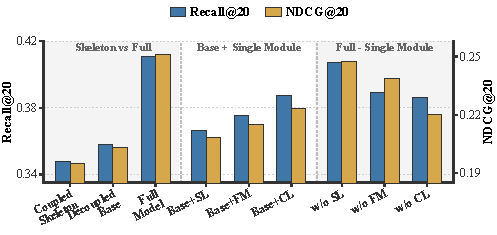
\includegraphics[width=\columnwidth]{image/ablation_chart_lastfm_unified}
	\caption{In-depth mechanism analysis on Last-FM, illustrating architecture evolution, additive gains, and subtractive impacts of key components.}
	\label{fig:ablation_chart_lastfm}
\end{figure}

\begin{figure*}[t] % 关键点：figure*
	\centering
	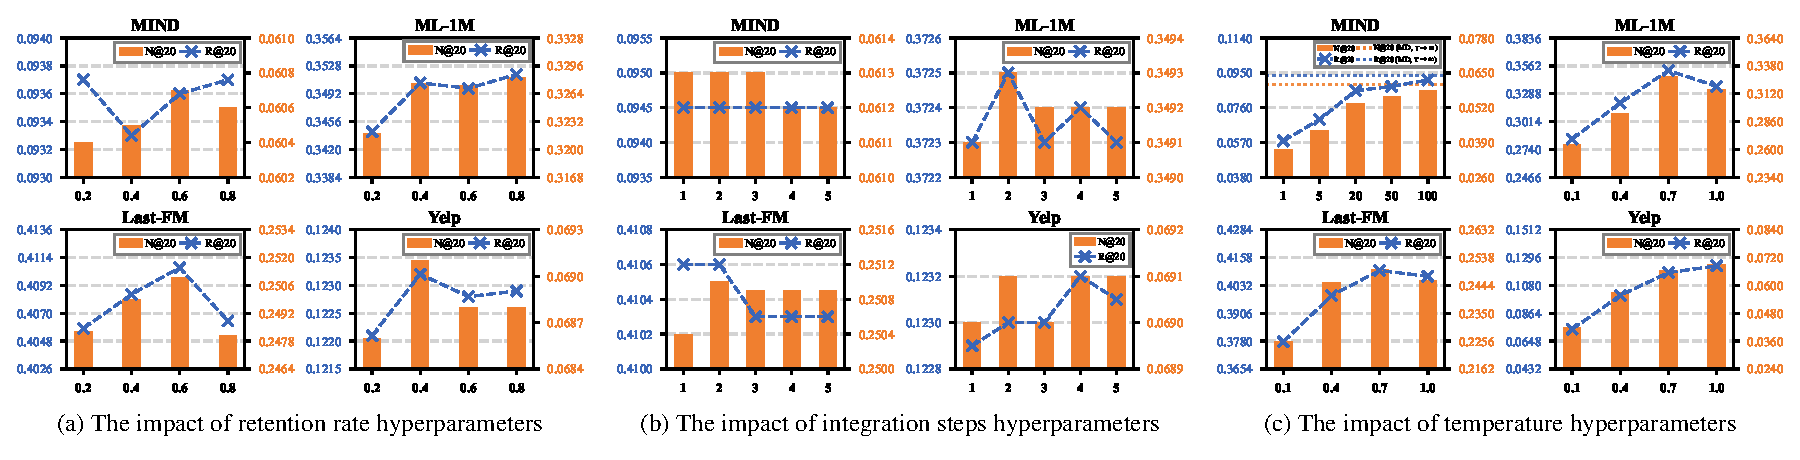
\includegraphics[width=1\textwidth]{image/hyperparameter_grid.pdf}
	\caption{Sensitivity analysis of key hyperparameters across four datasets, illustrating the impact of structure retention rate $\rho$, integration steps $N$, and contrastive temperature $\tau$. Dashed lines denote the theoretical performance limit using Mean Difference (MD) loss as $\tau \to \infty$.}
	\label{fig:hyperparameter}
\end{figure*}

\begin{figure}[t]
	\centering
	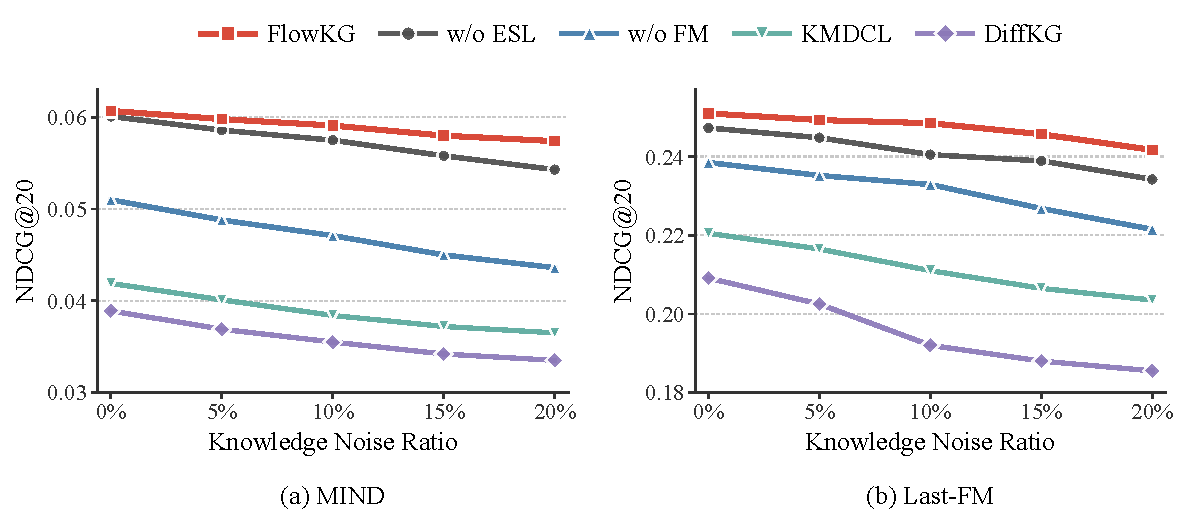
\includegraphics[width=\columnwidth]{image/noise_robustness}
	\caption{NDCG@20 under increasing knowledge noise ratios on MIND and Last-FM. The full FlowKG model is compared with its variants and representative baselines.}
	\label{fig:noise_robustness}
\end{figure}

\begin{figure}[t]
	\centering
	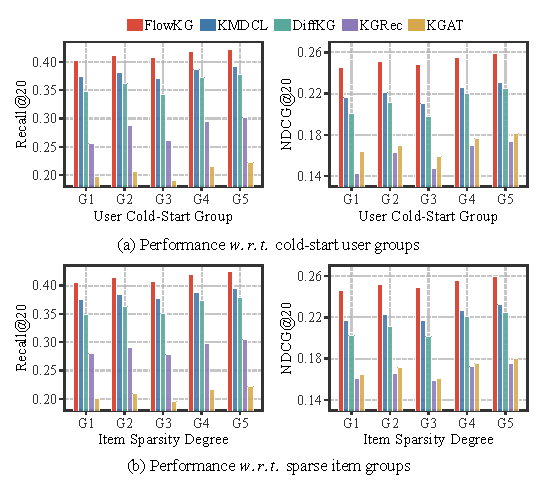
\includegraphics[width=\columnwidth]{image/lastfm_sparsity_metrics}
	\caption{Performance comparison across different user and item sparsity groups on Last-FM under NDCG@20 and Recall@20.}
	\label{fig:lastfm_sparsity_metrics}
\end{figure}

\begin{figure*}[t] % 星号 * 表示横跨双栏，[t] 表示通常建议放在页面顶部
	\centering
	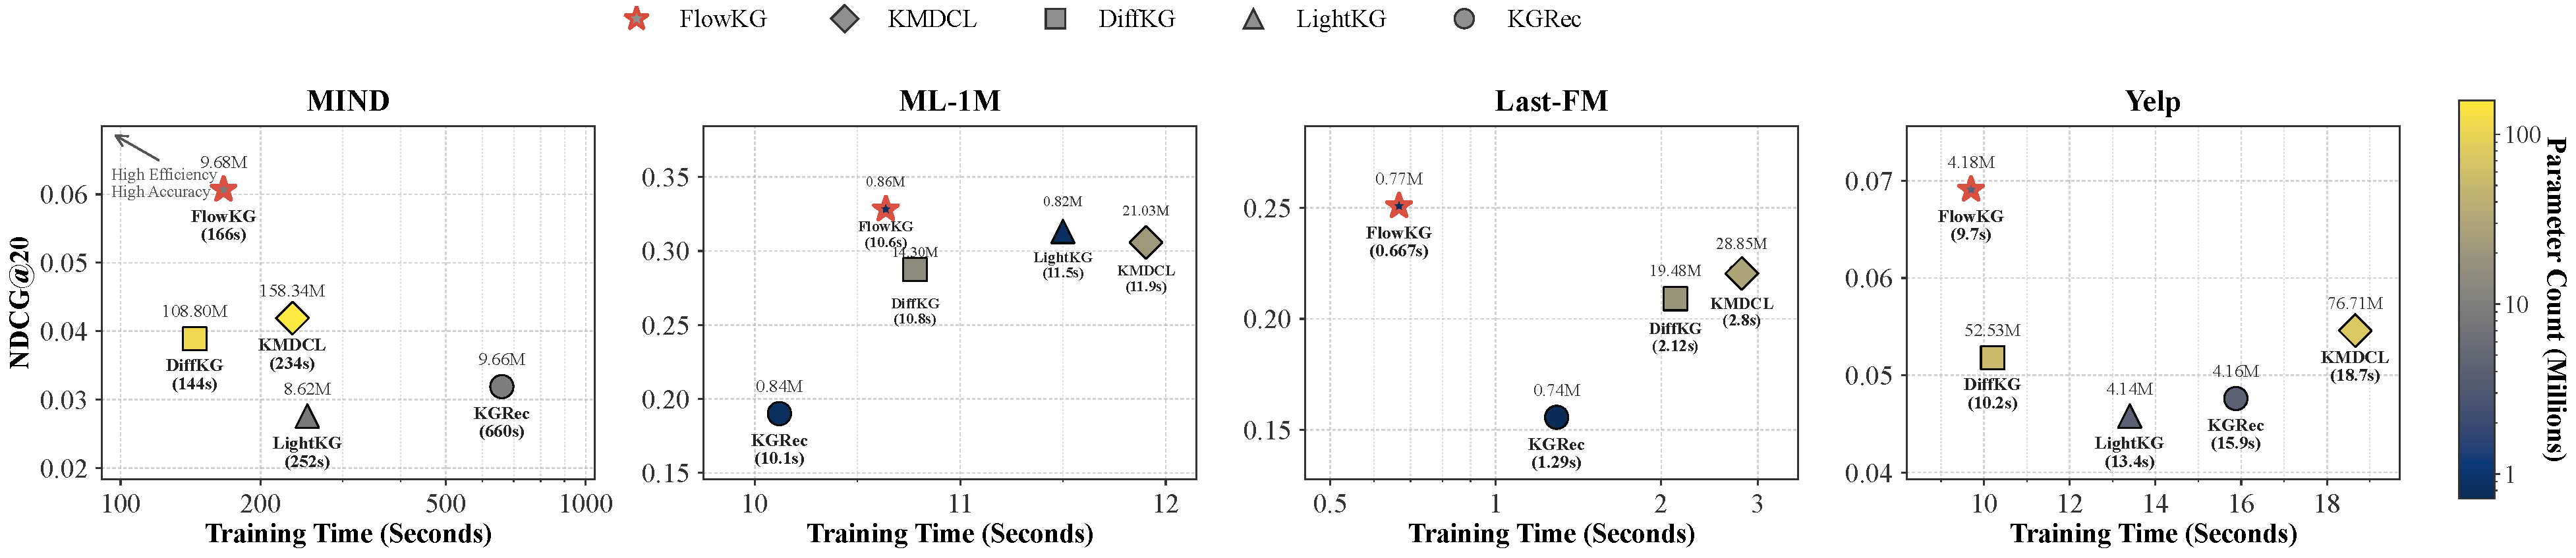
\includegraphics[width=1\textwidth]{image/efficiency_pareto.pdf} 
	% 使用 \textwidth 而不是 \columnwidth，因为你要跨越两栏
	\caption{Analysis of the trade-off between recommendation performance (NDCG@20) and training efficiency. The color intensity represents the model parameter scale, where FlowKG achieves the Pareto optimal balance across all datasets.}
	\label{fig:efficiency_pareto}
\end{figure*}

\iffalse
\begin{table}[t]
	\centering
	\caption{Tabular summary of the efficiency-performance trade-off in Figure~\ref{fig:efficiency_pareto}. Params denotes parameter count in millions, and Time denotes seconds per epoch.}
	\label{tab:efficiency_pareto}
	\scriptsize
	\setlength{\tabcolsep}{3.0pt}
	\renewcommand{\arraystretch}{1.05}
	\resizebox{\columnwidth}{!}{
		\begin{tabular}{llcccc}
			\toprule
			Methods & Component & MIND & ML-1M & Last-FM & Yelp \\
			\midrule
			\multirow{3}{*}{FlowKG}
			& NDCG@20 & \textbf{0.0607} & \textbf{0.3283} & \textbf{0.2509} & \textbf{0.0691} \\
			& Params (M) & 9.68 & 0.86 & 0.77 & 4.18 \\
			& Time (s) & 166.5 & 10.6 & 0.667 & 9.7 \\
			\midrule
			\multirow{3}{*}{KMDCL}
			& NDCG@20 & 0.0419 & 0.3059 & 0.2205 & 0.0546 \\
			& Params (M) & 158.34 & 21.03 & 28.85 & 76.71 \\
			& Time (s) & 234.0 & 11.9 & 2.8 & 18.7 \\
			\midrule
			\multirow{3}{*}{DiffKG}
			& NDCG@20 & 0.0389 & 0.2875 & 0.2091 & 0.0518 \\
			& Params (M) & 108.80 & 14.30 & 19.48 & 52.53 \\
			& Time (s) & 144.3 & 10.8 & 2.12 & 10.2 \\
			\midrule
			\multirow{3}{*}{LightKG}
			& NDCG@20 & 0.0276 & 0.3132 & 0.2430 & 0.0458 \\
			& Params (M) & 8.62 & 0.82 & 0.72 & 4.14 \\
			& Time (s) & 252.0 & 11.5 & 0.2 & 13.4 \\
			\midrule
			\multirow{3}{*}{KGRec}
			& NDCG@20 & 0.0319 & 0.1901 & 0.1556 & 0.0476 \\
			& Params (M) & 9.66 & 0.84 & 0.74 & 4.16 \\
			& Time (s) & 660.0 & 10.1 & 1.29 & 15.9 \\
			\bottomrule
		\end{tabular}
	}
\end{table}
\fi

\begin{figure}[t]
	\centering
	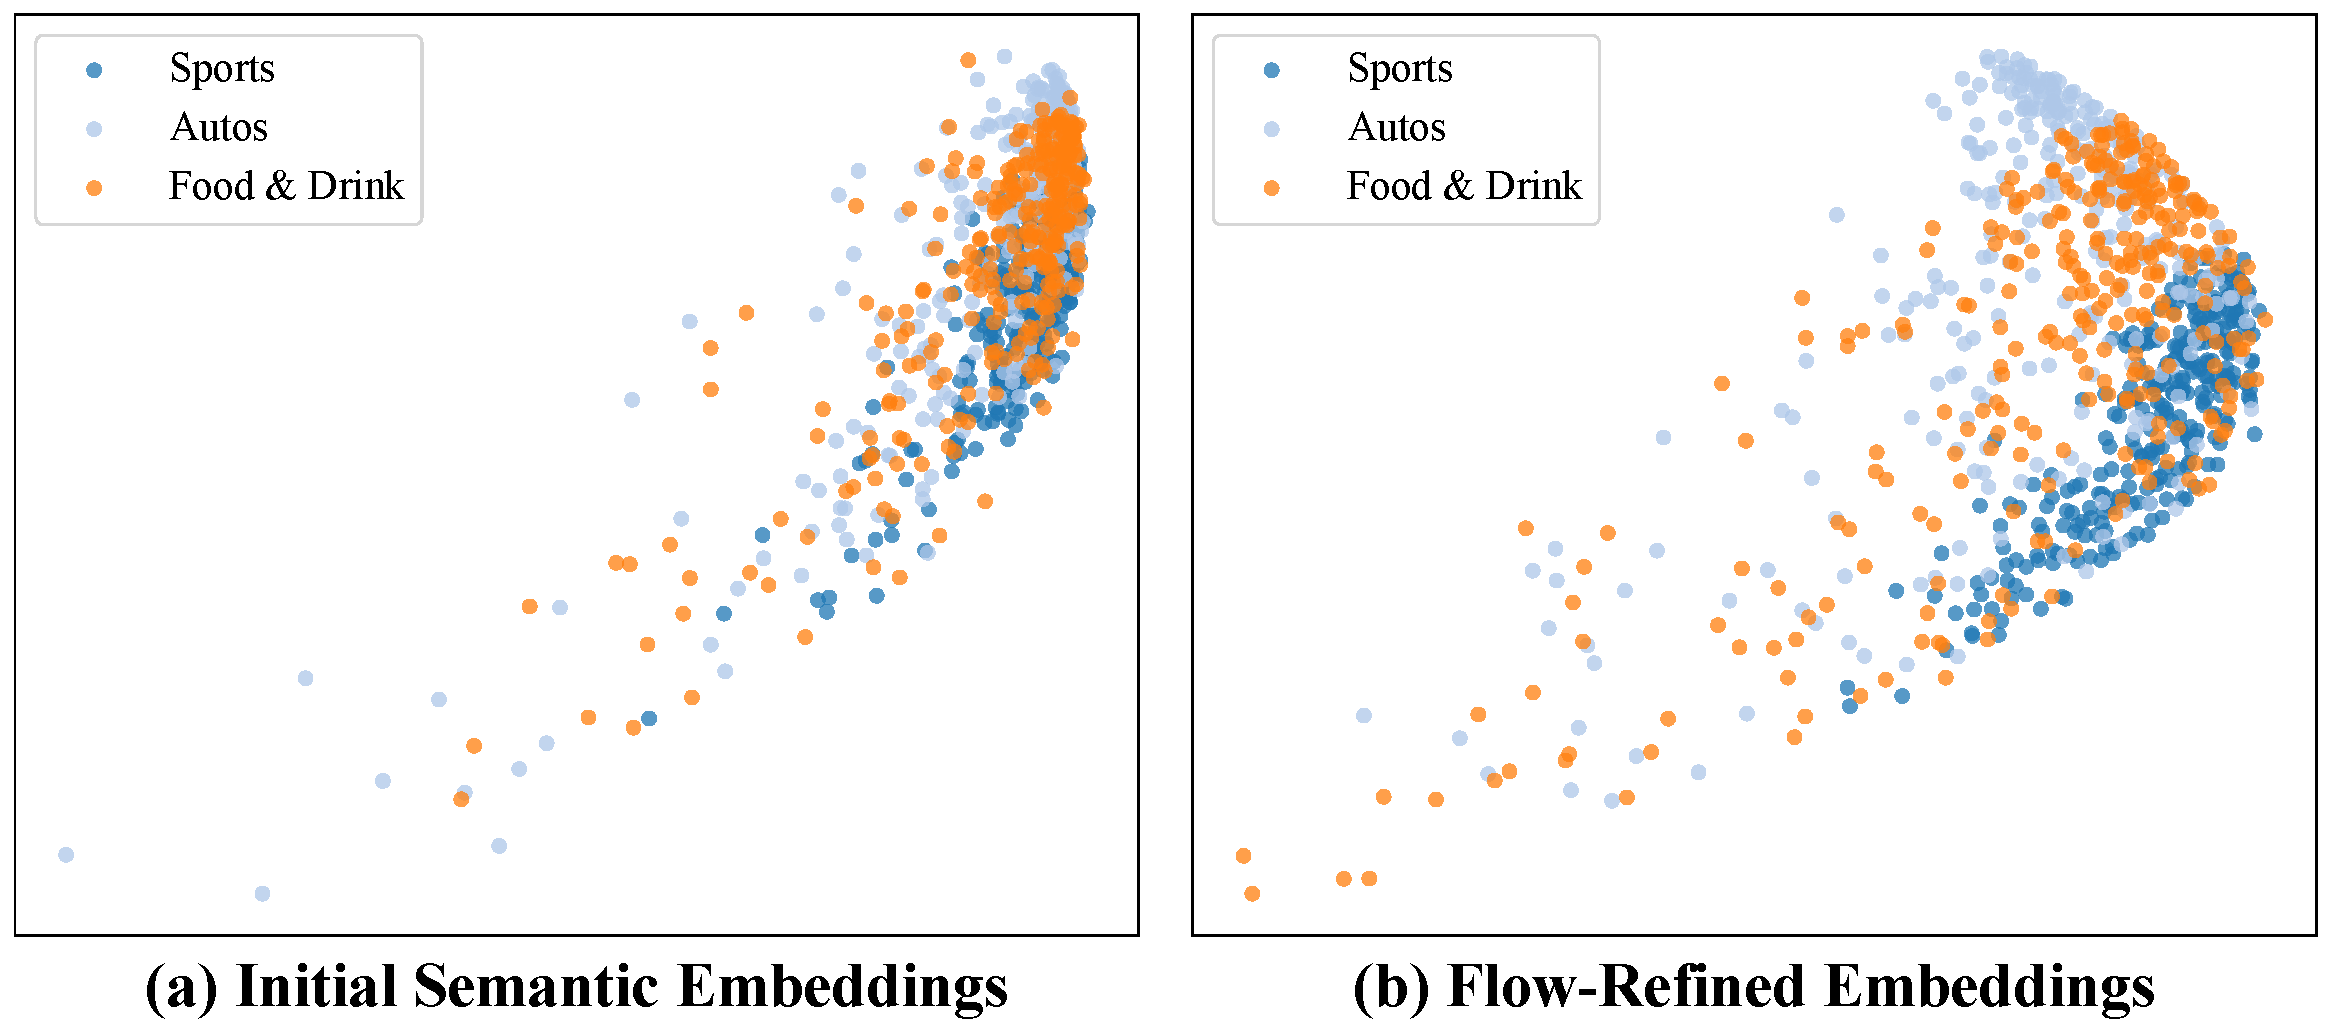
\includegraphics[width=\columnwidth]{image/scatter}
	\caption{Visualization of latent space evolution. (a) Initial embeddings exhibit severe semantic entanglement due to noise. (b) Flow-refined representations form compact, distinct clusters, demonstrating the effective recovery of semantic manifolds.}
	\label{fig:scatter}
\end{figure}



\subsection{Ablation Study (RQ2)}
\subsubsection{\textbf{Key Module Ablation}}
To systematically evaluate the contribution of each component, we compare the full FlowKG with four variants: (1) w/o ESL, removing the Entropy-Guided Structure Learning; (2) w/o DVE, replacing the Decoupled Dual-View Encoder with a coupled GNN architecture; (3) w/o FM, removing the Flow Matching Refinement; and (4) w/o CL, discarding the dual-level CL. For compact presentation, the main text reports three representative datasets in Table~\ref{tab:ablation}, with the complete four-dataset ablation results provided in Appendix~\ref{app:full_ablation}. Figure~\ref{fig:ablation_chart_lastfm} further analyzes the Last-FM mechanism.


Table~\ref{tab:ablation} confirms the full model's superior performance, demonstrating module synergy. First, removing CL causes the most severe degradation (e.g., -34.7\% Recall@20 on MIND), establishing it as a foundational paradigm against data sparsity. Furthermore, the substantial drop without FM verifies its critical role in preventing representation degradation through distributional evolution. Finally, the consistent performance losses without ESL and DVE confirm that filtering structural noise and decoupling views are essential prerequisites for robust representation learning.

Figure~\ref{fig:ablation_chart_lastfm} presents a multi-dimensional ablation study on Last-FM to scrutinize the internal mechanism. The Decoupled Skeleton outperforms the Coupled Skeleton in Recall@20 (0.352 vs. 0.342), empirically validating that strict view decoupling prevents noise propagation. Both additive and subtractive analyses confirm the contribution of each component: adding ESL, FM, or CL individually improves performance, while removing any causes decline. This consistent "building-up" and "stripping-down" evidence robustly verifies that every module in FlowKG distinctively enhances the final performance.

\subsubsection{\textbf{Sensitivity to Key Hyperparameters}}
To investigate the properties of FlowKG, we analyze the impact of three key hyperparameters: the retention rate $\rho$, integration steps $N$, and contrastive temperature $\tau$, as summarized in Figure~\ref{fig:hyperparameter}.


\noindent\textbf{Impact of Retention Rate $\rho$.}
As shown in Figure~\ref{fig:hyperparameter}(a), performance follows a convex pattern across all datasets. Both excessive pruning ($\rho=0.1$) and retaining the full noisy graph ($\rho \to 1.0$) lead to degradation. The optimal sweet spot typically spans from $\rho=0.4$ to $\rho=0.8$, confirming that the Entropy-Guided Structure Learning module successfully identifies a trade-off zone where structural noise is filtered while intrinsic semantic information is preserved.

\noindent\textbf{Impact of Integration Steps $N$.}
Figure~\ref{fig:hyperparameter}(b) demonstrates the remarkable stability of our Flow Matching mechanism. Notably, the model achieves optimal performance within just 1--3 Euler steps, and performance remains consistently stable beyond this point. This implies that the learned vector field constructs a highly straight ODE trajectory in the latent space, allowing the model to jump from noise to the target manifold directly. Consequently, a minimal number of integration steps is sufficient for inference, ensuring maximal computational efficiency without sacrificing accuracy.

\noindent\textbf{Impact of Temperature $\tau$.}
Figure~\ref{fig:hyperparameter}(c) reveals dataset-dependent preferences. Denser datasets like ML-1M benefit from a moderate $\tau$ (e.g., 0.2) to maintain discriminative power. Conversely, on the MIND dataset characterized by extreme interaction sparsity and high-dimensional relations, performance improves monotonically as $\tau$ increases, peaking at the theoretical limit of Mean Difference (MD) loss. This verifies that in scenarios with high sparsity where ``hard negatives'' are likely to be unobserved positives (False Negatives), shifting the objective from local hard-negative discrimination to global representation alignment (via high $\tau$ or MD loss) provides significantly better robustness.

\subsection{Robustness Analysis (RQ3)}


To evaluate robustness against structural perturbations, we inject random KG noise at ratios from 0\% to 20\%. As shown in Figure~\ref{fig:noise_robustness}, FlowKG consistently achieves the best NDCG@20 and degrades more slowly than KMDCL and DiffKG. Removing either ESL or FM reduces robustness, with the gap widening as noise increases. These results confirm that upstream structure filtering and downstream representation refinement provide complementary protection against noisy knowledge.

We further examine robustness under different sparsity conditions on Last-FM. As shown in Figure~\ref{fig:lastfm_sparsity_metrics}, FlowKG maintains consistent advantages across both user and item groups under NDCG@20 and Recall@20, indicating that the proposed decoupled structure learning and flow-based refinement remain effective for sparse recommendation scenarios.

%\begin{figure}[t]
%	\centering
%	\includegraphics[width=\linewidth]{image/case_study} % 插入你的图片文件
%	\caption{Case Study on MovieLens-1M for item \textbf{``Interstellar''}.}
%	\label{fig:case_study}
%\end{figure}

\subsection{Computational Efficiency Analysis (RQ4)}


To investigate the trade-off between recommendation accuracy and resource consumption, we visualize the relationship between NDCG@20, training time (per epoch), and parameter magnitude in Figure~\ref{fig:efficiency_pareto}.
FlowKG demonstrates a superior Pareto efficiency, achieving SOTA performance while maintaining low computational overhead.
In terms of model complexity, FlowKG achieves a significant reduction in parameter count compared to other generative baselines like DiffKG and KMDCL, aligning closely with lightweight discriminative models such as LightKG and KGRec.
This efficiency stems from our design choice to conduct generation in the latent space rather than the graph space.
While KMDCL performs diffusion on the high-dimensional graph structure $\mathbb{R}^{|\mathcal{E}| \times |\mathcal{E}|}$, FlowKG operates strictly within the compact item representation space $\mathbb{R}^{|\mathcal{I}| \times d}$.
This dimensional reduction circumvents the prohibitive parameter costs associated with graph-level generation.
Regarding temporal efficiency, FlowKG consistently ranks in the top tier across diverse datasets.
Unlike SDE-based diffusion models that require computationally expensive stochastic sampling and extensive denoising steps, our Flow Matching framework utilizes a deterministic ODE solver.
This enables rapid convergence during training and efficient inference, successfully reconciling the high expressiveness of generative models with the practicality required for large-scale recommendation.

\subsection{Visual Interpretability of Manifold Evolution (RQ5)}


To intuitively verify the efficacy of the Flow Matching module in rectifying latent representations, we visualize the evolution of item embeddings using Principal Component Analysis (PCA), as depicted in Figure~\ref{fig:scatter}. In the initial state (Figure~\ref{fig:scatter}a), embeddings from distinct categories (e.g., Sports, Autos) exhibit severe semantic entanglement with blurred decision boundaries. This observation confirms that despite the structural pruning, the raw semantic encoder remains susceptible to residual noise, resulting in a dispersed distribution. Conversely, after undergoing the flow-based refinement (Figure~\ref{fig:scatter}b), the representations evolve into compact, well-separated clusters with clear manifold structures. This distinct separation demonstrates that the learned deterministic ODE trajectory successfully acts as a "semantic rectifier," guiding item embeddings from a disordered, noisy distribution to a structured high-density region, thereby significantly enhancing their discriminative power for downstream recommendation.



\section{Conclusion}
\label{sec:conclusion}

In this work, we address the noise propagation issue in cascaded architectures and the computational challenges of diffusion-based generative methods. To tackle these, we propose FlowKG, a robust framework featuring a Decoupled Dual-View Encoder and an Entropy-Guided Structure Learning module that combines structural priors with semantic posteriors for principled, fine-grained graph denoising. Crucially, we introduce Flow Matching to the knowledge graph-based recommendation task, utilizing deterministic Ordinary Differential Equation paths to efficiently refine latent item representations via Optimal Transport. Extensive experimental results demonstrate FlowKG's superior performance in accuracy, training efficiency, and robustness against structural noise.

%For future work, we plan to explore the synergy between Flow Matching and Large Language Models (LLMs). We aim to leverage the rich semantic reasoning capabilities of LLMs to construct high-fidelity initial semantic spaces, thereby further enhancing the quality and explainability of the generative process.

\bibliography{sigir2026}

\appendix
\setcounter{secnumdepth}{1}
\section{Derivation of Relation Branching Entropy}
\label{app:relation_entropy}

The relation entropy prior aims to measure the structural branching uncertainty of each relation \(r\). Given a head entity \(h\) and a relation \(r\), we denote the corresponding tail entity set as
\begin{equation}
\label{eq:app_tail_set}
\mathcal{N}_{h}^{r}=\{t \mid (h,r,t)\in \mathcal{G}_{kg}\}.
\end{equation}

We first consider the local uncertainty of tail selection conditioned on a specific head-relation pair \((h,r)\):
\begin{equation}
\label{eq:app_local_entropy}
H(T\mid h,r)
=
-\sum_{t\in \mathcal{N}_{h}^{r}}p(t\mid h,r)\log p(t\mid h,r).
\end{equation}

Here, the conditional distribution is defined over the local tail set \(\mathcal{N}_{h}^{r}\) after the head entity \(h\) and relation \(r\) are specified. It measures how dispersed the reachable tail entities are within this local neighborhood, rather than characterizing the global tail distribution \(p(t\mid r)\) of relation \(r\) over the entire knowledge graph.

In standard knowledge graphs, triples are usually unweighted, meaning that the graph only indicates whether a triple exists, without providing edge weights, occurrence frequencies, or confidence scores for different tails under the same \((h,r)\). Therefore, in the absence of additional probabilistic information, we adopt a local maximum-entropy prior and treat the observed tail entities in \(\mathcal{N}_{h}^{r}\) as equally likely neighbors:
\begin{equation}
\label{eq:app_local_uniform_prior}
p(t\mid h,r)=\frac{1}{|\mathcal{N}_{h}^{r}|}.
\end{equation}

Substituting this local prior into the conditional entropy gives:
\begin{equation}
\label{eq:app_entropy_derivation}
\begin{aligned}
	H(T\mid h,r)
	&=
	-\sum_{t\in \mathcal{N}_{h}^{r}}
	\frac{1}{|\mathcal{N}_{h}^{r}|}
	\log \frac{1}{|\mathcal{N}_{h}^{r}|} \\
	&=
	-|\mathcal{N}_{h}^{r}|
	\cdot
	\frac{1}{|\mathcal{N}_{h}^{r}|}
	\log \frac{1}{|\mathcal{N}_{h}^{r}|} \\
	&=
	\log |\mathcal{N}_{h}^{r}|.
\end{aligned}
\end{equation}

Thus, the conditional entropy of a given head-relation pair reduces to the logarithm of its branching factor. A larger value means that more tail entities can be reached from \(h\) through relation \(r\), indicating higher local structural uncertainty.

To obtain a relation-level measure, we aggregate the local branching entropy over all head entities associated with relation \(r\). Let
\begin{equation}
\label{eq:app_head_set}
\mathcal{H}_{r}
=
\{h \mid \exists t,\ (h,r,t)\in \mathcal{G}_{kg}\}.
\end{equation}
The branching entropy of relation \(r\) is then defined as:
\begin{equation}
\label{eq:app_relation_branching_entropy}
H(r)
=
\frac{1}{|\mathcal{H}_{r}|}
\sum_{h\in \mathcal{H}_{r}}
\log |\mathcal{N}_{h}^{r}|.
\end{equation}

Finally, we normalize the inverse entropy to obtain the structural prior score:
\begin{equation}
\label{eq:app_relation_entropy_prior}
S_{\mathrm{prior}}(r)
=
1-\frac{H(r)}{\max_{r'\in\mathcal{R}}H(r')}.
\end{equation}

A larger \(S_{\mathrm{prior}}(r)\) indicates lower structural branching uncertainty and higher prior reliability. This prior is later combined with the triplet-level semantic score to guide knowledge graph structure filtering.


\end{document}
